\documentclass[rbe,wwwview]{econbr}

%%%%%%%%%%%%%%%%%%%%%%%%%%%%%%%%
% ISSUE CONFIGURATION [START] (you don't have to worry about these)
%%%%%%%%%%%%%%%%%%%%%%%%%%%%%%%%
\usepackage[contents={Versão\ submissão},color=black!15,angle=45,scale=6,hshift=17pt,firstpage=TRUE]{background}
\usepackage{float}      % para [H]
\usepackage{graphicx}   % para \scalebox
\usepackage{booktabs}   % para \toprule, \midrule, \bottomrule, \cmidrule
\usepackage{caption}    % para \caption*, \captionsetup
\usepackage{makecell}   % para \makecell

\renewcommand{\fonte}[1]{
    \begin{center}
    \footnotesize
    Fonte: #1
    \end{center}
}
\startlocaldefs
\def\@volume{1} % Edition Volume
\def\@issue{1} % Edition Number
\def\@pubyear{202x} % Year of publication
\def\@doi{xxxx} % Article DOI (WITHOUT the prefix https://doi.org/)
\def\@firstpage{1} % Article starting page. Must be configured manually
\def\@lastpage{1} % Article final page. Must be configured manually
\def\@received{x month, 202x} % Manuscript submitted on...
\def\@accepted{x month, 202x} %  Manuscript accepted on...
\def\@pubonline{x month, 202x} % Published online on... (Must be configured manually)
\setcounter{page}{\@firstpage}
\coeditor{} % Co-editor responsible for handling the submitted manuscript
\def\@runauthor{Gonçalves et al.} %% RUNNING AUTHOR NAMES (appears on header every other page)
\patchcmd\author@fmt{\def\ead}{\let\orcidlink\@gobble\def\ead}{}{}
\endlocaldefs
%%%%%%%%%%%%%%%%%%%%%%%%%%%%%%%%
% ISSUE CONFIGURATION [END] (you don't have to worry about these)
%%%%%%%%%%%%%%%%%%%%%%%%%%%%%%%%

%%%%%%%%%%%%%%%%%%%%%%%%%%%%%%%%
% Package siunitx configuration:
%%%%%%%%%%%%%%%%%%%%%%%%%%%%%%%%
\sisetup{
detect-mode,
% parse-numbers = false,
output-decimal-marker={.},
tight-spacing = true,
group-digits = false,
input-signs = -,
input-open-uncertainty = ,
input-close-uncertainty = ,
table-align-text-pre = false,
table-align-text-after = false,
round-mode = places,
round-precision = 2, % default rounding in tables with column-type S
table-space-text-pre = (,
table-space-text-post = ),
}

%%%%%%%%%%%%%%%%%%%%%%%%%%%%%%%%%%%%%
%% Please load custom packages below:
%%%%%%%%%%%%%%%%%%%%%%%%%%%%%%%%%%%%%
% \usepackage{tikz}

\begin{document}
%\selectlanguage{english}
\selectlanguage{brazil}
\begin{frontmatter}

%% ARTICLE TITLE
\title{Tendências regionais do mercado de trabalho em Minas Gerais: estimativas baseadas em modelos para os estratos geográficos da PNAD Contínua}

%% ARTICLE RUNNING TITLE (appears on header every other page)
\runtitle{Tendências do mercado de trabalho nos estratos geográficos}

\begin{aug}
% use \particle for den|der|de|van|von (only lc!)
% [id=?,addressref=?,corref]{\fnms{}~\snm{}\ead[label=e?]{}\thanksref{}}
%
%% e-mail is mandatory for each author
%
%%% initials in fnms (if any) with spaces
%
%% FIRST AUTHOR:
\author[id=au1,addressref={add2}]{%
  \fnms{Paulo Roberto Betbeder}~\snm{Gonçalves}%
  \orcidlink{0009-0002-9474-8476}%
  \ead[label=e1]{paulogon13@gmail.com }
}
%% SECOND AUTHOR:
\author[id=au2,addressref={add3}]{%
  \fnms{Caio César Soares}~\snm{Gonçalves}%
  \orcidlink{0000-0002-3366-7560}%
  \ead[label=e2]{ccsgonc@gmail.com}
}
%% THIRD AUTHOR:
\author[id=au3,addressref={add1}]{%
  \fnms{Nícia Raies Moreira de}~\snm{Souza}%
  \orcidlink{0000-0002-4069-9560}%
  \ead[label=e3]{nicia.raies@fjp.mg.gov.br}
}
%% FOURTH AUTHOR:
\author[id=au4,addressref={add5}]{%
  \fnms{Denise Britz do Nascimento}~\snm{Silva}%
  \orcidlink{0000-0002-5514-7558}%
  \ead[label=e4]{denisebritz@gmail.com}
}
%% FIFTH AUTHOR:
\author[id=au5,addressref={add4}]{%
  \fnms{Luna}~\snm{Hidalgo}%
  \orcidlink{0000-0000-0000-0000}%
  \ead[label=e5]{lunahidalgo@gmail.com}
}
%% and so on.

%%%%%%%%%%%%%%%%%%%%%%%%%%%%%%%%%%%%%%%%%%%%%%
%% ADDRESSES                                %%
%%%%%%%%%%%%%%%%%%%%%%%%%%%%%%%%%%%%%%%%%%%%%%
%% FUNDAÇÃO JOÃO PINHEIRO
\address[id=add1]{%
  \orgdiv{Diretoria de Estatística e Informações},
  \orgname{Fundação João Pinheiro},
  \city{Belo Horizonte},
  \state{MG, Brasil}
}

%% UNIVERSIDADE FEDERAL DE JUIZ DE FORA
\address[id=add2]{%
  \orgdiv{Departamento de Economia},
  \orgname{Universidade Federal de Juiz de Fora},
  \city{Juiz de Fora},
  \state{MG,Brasil}
}

%% UFMG
\address[id=add3]{%
  \orgdiv{Departamento de Demografia},
  \orgname{Universidade Federal de Minas Gerais},
  \city{Belo Horizonte},
  \state{MG,Brasil}
}

%% CONSULTORA INDEPENDENTE
\address[id=add4]{%
  \orgname{Consultora independente},
  \city{Madrid,Espanhã}
}

%% SCIENCE
\address[id=add5]{%
  \orgname{SCIENCE},
  \city{Rio de Janeiro},
  \state{RJ,Brasil}
}
\end{aug}

%% SUPPORT INFO (Reminder: do not thank the handling coeditor anonymously or by name)
%% \support{We thank four anonymous referees. The Editor should not be thanked anonymously or by name in this footnote, or elsewhere in the paper. The first author gratefully acknowledges financial support from the National Science Foundation through Grant XXX-0000000.}

%% ABSTRACT:
\begin{abstract}
Este artigo analisa as tendências do total de desocupados, do total de ocupados e da taxa de desocupação nos estratos geográficos de Minas Gerais, com dados trimestrais da PNAD Contínua de 2012 a 2024. Para lidar com a maior variabilidade amostral em domínios desagregados, empregam-se modelos estruturais em espaço de estados com incorporação explícita do erro amostral. Os resultados indicam que as estimativas baseadas em modelo preservam a trajetória das estimativas diretas e apresentam ganhos de precisão, reforçando o potencial da modelagem para produzir estatísticas regionais do mercado de trabalho.
\end{abstract}

\begin{abstract}[Abstract]
This article analyzes trends in the number of unemployed persons, employed persons, and the unemployment rate across geographic strata of Minas Gerais, using quarterly data from the Continuous PNAD from 2012 to 2024. To address higher sampling variability in disaggregated domains, we employ structural state-space models with explicit incorporation of sampling error. The results indicate that model-based estimates preserve the trajectory of direct estimates while improving precision, reinforcing the potential of time series modeling for producing regional labor market statistics.
\end{abstract}

%% KEYWORDS:
\begin{keyword}
\kwd{Mercado de trabalho}
\kwd{Desemprego}
\kwd{Estimação em pequenas áreas}
\kwd{Modelos em espaço de estados}
\end{keyword}

\begin{keyword}[class=JEL]
\kwd{C32}
\kwd{C53}
\kwd{J64}
\end{keyword}

\end{frontmatter}

%%%%%%%%%%%%%%%%%%%%%%%%%%%%%%%%%%%%%%%%%%%%%%%%%%%%%%%%%%%%%%%%%%%%%%%%%
%%%% MAIN TEXT ENTRY AREA:
%%%%%%%%%%%%%%%%%%%%%%%%%%%%%%%%%%%%%%%%%%%%%%%%%%%%%%%%%%%%%%%%%%%%%%%%%

\section{Introdução}\label{sec:Introdução}

A Pesquisa Nacional por Amostra de Domicílios Contínua (PNAD Contínua) constitui a principal fonte de informações conjunturais sobre o mercado de trabalho brasileiro. Seus resultados permitem acompanhar a evolução da ocupação, da desocupação e de outros indicadores associados à inserção da população na força de trabalho. No caso de Minas Gerais, a taxa de desocupação atingiu 4,3\% no quarto trimestre de 2024, acompanhando a trajetória de queda observada no país desde 2021 \citep{ibge2025pnad}. Contudo, o comportamento agregado estadual pode ocultar dinâmicas regionais bastante distintas, especialmente em uma unidade da federação marcada por grande extensão territorial, elevado número de municípios e forte heterogeneidade socioeconômica \citep{ibgecidades}.

A partir de abril de 2022, o Instituto Brasileiro de Geografia e Estatística (IBGE) passou a divulgar resultados da PNAD Contínua desagregados por estrato geográfico, em caráter experimental \citep{ibge_estratos,ibge_experimental}. Essa classificação indica que tais estatísticas ainda se encontram em processo de consolidação metodológica e institucional, estando sujeitas a avaliações contínuas quanto à sua consistência, precisão e potencial de uso analítico, conforme também previsto nas diretrizes internacionais para a produção de estatísticas experimentais \citep{eurostat_experimental}.

Essa ampliação da divulgação territorial dialoga com uma demanda recorrente no campo das estatísticas públicas: produzir informações mais oportunas, mais desagregadas e com precisão suficiente para orientar decisões em diferentes escalas territoriais. Como discutido em \citet{goncalves2023tese}, a expansão da produção estatística no espaço pode ser compreendida como uma forma de aproveitar pesquisas amostrais repetidas já consolidadas, combinando a abordagem baseada no desenho amostral com métodos baseados em modelos. No caso da PNAD Contínua, esse debate é especialmente relevante porque a pesquisa possui periodicidade contínua e desenho com painéis rotativos, o que permite explorar a acumulação de informação no tempo para melhorar a precisão de estimativas em domínios menores.

A principal limitação para o uso analítico dessas estimativas em domínios mais desagregados decorre da redução do tamanho efetivo da amostra. À medida que o domínio de interesse se restringe, as estimativas diretas passam a apresentar maior variância, intervalos de confiança mais amplos e coeficientes de variação mais elevados. Esse problema é amplamente reconhecido na literatura de estimação em pequenas áreas, na qual métodos baseados exclusivamente no desenho amostral tendem a perder precisão quando aplicados a subpopulações ou recortes territoriais de menor dimensão \citep{rao2015}. No caso da PNAD Contínua, essa limitação se manifesta em coeficientes de variação que, em alguns estratos e períodos, aproximam-se ou ultrapassam o patamar de 30\% adotado pelo IBGE como referência para alta imprecisão \citep{ibgecv,ibge_estratos}.

Nesse contexto, a literatura tem destacado o potencial de modelos de séries temporais para pesquisas amostrais repetidas como alternativa para aprimorar a precisão de indicadores produzidos em domínios menores. A ideia central consiste em decompor a série observada em dois componentes: populacional (não observado) e erro amostral, permitindo separar a dinâmica subjacente do fenômeno de interesse do ruído decorrente do processo de amostragem \citep{scott1974,scott1977,smith,harvey1989}. Aplicações dessa abordagem foram desenvolvidas para estimativas subnacionais do mercado de trabalho nos Estados Unidos \citep{tiller2006}, nos Países Baixos \citep{brakel2016,boonstra2019} e no Reino Unido \citep{ons_experimental,elliott2019}. No Brasil, \citet{goncalves2022} aplicaram modelos em espaço de estados à taxa de desocupação mensal da PNAD Contínua, em níveis nacional e estadual, obtendo estimativas mais precisas que as estimativas diretas. O presente artigo avança nessa agenda ao deslocar o foco para domínios intraestaduais, analisando os estratos geográficos de Minas Gerais.

Estudos recentes com a PNAD Contínua têm explorado a dinâmica do desemprego no Brasil a partir de diferentes perspectivas. \citet{borges2024} analisam o desemprego de longa duração e discutem a persistência na condição de desocupado, enquanto \citet{guinesi2026} utilizam a estrutura longitudinal da pesquisa para acompanhar transições individuais no mercado de trabalho entre 2012 e 2021. Diferentemente desses estudos, este artigo não acompanha trajetórias individuais, mas analisa a evolução temporal de indicadores regionais, buscando produzir estimativas mais estáveis para domínios intraestaduais.

Diante da escassez de indicadores regionais confiáveis e da crescente demanda por informações capazes de captar as heterogeneidades territoriais do mercado de trabalho, este estudo tem como objetivo analisar as tendências das séries do total de desocupados, do total de ocupados e da taxa de desocupação nos estratos geográficos de Minas Gerais. Embora indicadores consolidados estejam disponíveis para o Brasil e para as unidades da federação, a produção sistemática de estatísticas consistentes em níveis intraestaduais ainda enfrenta limitações importantes, sobretudo em razão da elevada variabilidade das estimativas diretas em domínios mais desagregados. Para isso, utilizam-se séries trimestrais da PNAD Contínua no período de 2012 a 2024, buscando oferecer uma leitura de longo prazo da dinâmica regional do mercado de trabalho no estado.

No Brasil, a dimensão regional do desemprego já foi objeto de estudos voltados à análise de convergência das taxas de desemprego entre regiões \citep{ferrari2015}. No caso específico de Minas Gerais, iniciativas recentes buscaram ampliar a leitura temporal da desocupação por meio da compatibilização entre diferentes pesquisas domiciliares \citep{marques2024}. O presente artigo dialoga com essa literatura ao deslocar o foco para a dimensão intraestadual, explorando os estratos geográficos da PNAD Contínua e utilizando modelos estruturais para reduzir a variabilidade das estimativas diretas em domínios menores.

A principal contribuição do artigo é oferecer evidências sobre a dinâmica regional do mercado de trabalho mineiro a partir de estimativas mais precisas para domínios intraestaduais da PNAD Contínua. Para isso, empregam-se modelos estruturais em espaço de estados capazes de estimar simultaneamente os componentes não observados das séries e o erro amostral associado ao desenho da pesquisa. O artigo contribui, assim, para a literatura de economia aplicada ao combinar análise regional do mercado de trabalho, mensuração de indicadores econômicos e métodos de séries temporais para pesquisas amostrais repetidas.

Além desta introdução, o artigo está organizado em quatro seções. A Seção \ref{sec:estratos} descreve os estratos geográficos de Minas Gerais e discute a precisão das estimativas diretas da PNAD Contínua. A Seção \ref{sec:metodologia} apresenta a base de dados e a estratégia metodológica adotada. A Seção \ref{sec:resultados} discute os principais resultados empíricos, com ênfase na comparação entre estimativas diretas e estimativas baseadas em modelo. Por fim, a Seção \ref{sec:conclusão} apresenta as considerações finais.

\section{Os estratos geográficos de Minas Gerais}
\label{sec:estratos}

A regionalização adotada neste artigo decorre dos estratos geográficos definidos na amostra mestra do Sistema Integrado de Pesquisas Domiciliares (SIPD) do IBGE \citep{freitasantonaci2010}. Segundo essa estrutura, Minas Gerais é composto por dez estratos geográficos, que correspondem à capital e a nove grupos de municípios. Esses recortes foram originalmente definidos para fins de planejamento e operacionalização da amostra, mas também permitem explorar diferenças territoriais relevantes no interior do estado.

Neste estudo, os dez estratos originais foram reorganizados em oito regiões de análise. Essa decisão decorreu da combinação da RIDE de Brasília em Minas com o Norte de Minas Gerais e do Colar Metropolitano de Belo Horizonte com o Entorno Metropolitano de Belo Horizonte. A Figura \ref{fig:figestratos} apresenta a divisão territorial conforme definição da SIPD.

\vspace{-1em}

\begin{figure}[H]
    \centering
     \caption{Divisão dos estratos geográficos de Minas Gerais conforme SIPD}
    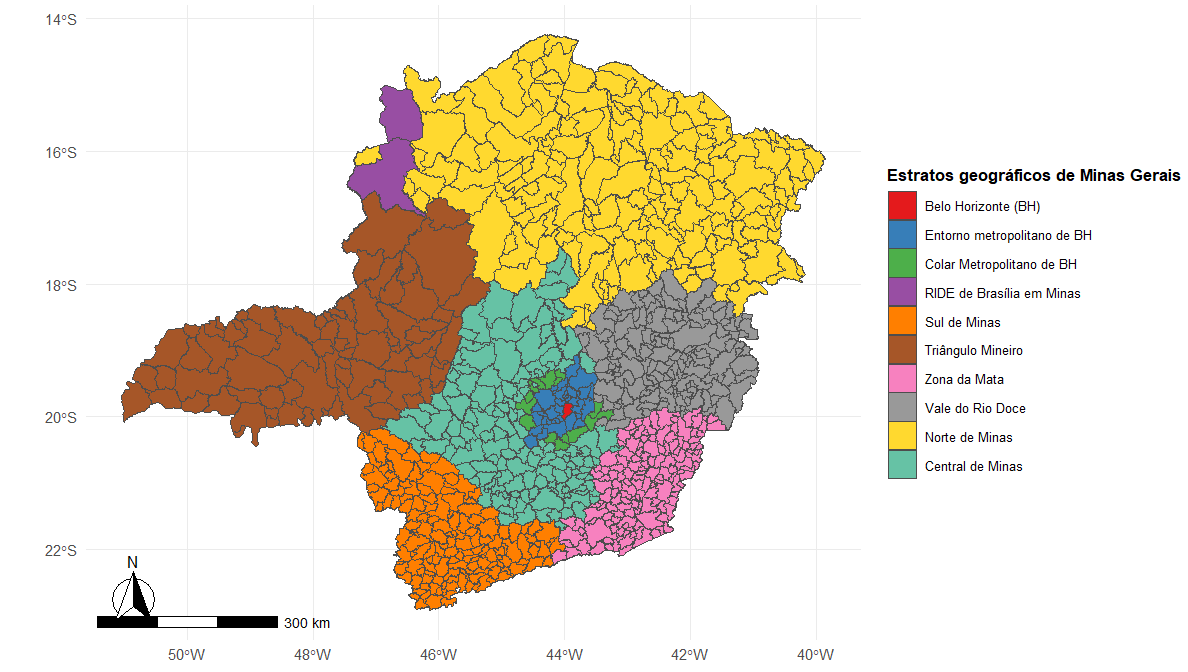
\includegraphics[width=0.8\linewidth]{Figs estratos/estratos minas.png}
    \fonte{Elaboração própria, com base nos dados da PNAD Contínua. Nota: Projeção de Albers, Datum: WGS 84, EPSG: 4674 -- SIRGAS 2000.}
    \label{fig:figestratos}
\end{figure}


A agregação desses estratos foi motivada pela elevada imprecisão das estimativas diretas nas duas menores regiões, especialmente na série do total de desocupados. Além do critério estatístico, consideraram-se também a proximidade geográfica e a estrutura de influência regional das cidades, conforme a Região de Influência das Cidades (REGIC) \citep{ibgeregic2018}.

A Figura \ref{fig:cvregs} ilustra a evolução dos coeficientes de variação das estimativas diretas do total de desocupados para os dez estratos originais. Observa-se que, após 2019, tanto a RIDE de Brasília em Minas quanto o Colar Metropolitano de Belo Horizonte apresentaram coeficientes de variação sistematicamente superiores aos dos demais estratos. Em determinados trimestres, os coeficientes de variação dessas regiões ultrapassaram o patamar de 30\%, considerado pelo IBGE como indicativo de alta imprecisão \citep{ibge2022nota}.

\vspace{-2em}

\begin{figure}[H]
    \centering
    \caption{Evolução do coeficiente de variação do total de desocupados -- dez estratos originais -- 1º trimestre de 2012 ao 2º trimestre de 2024}
    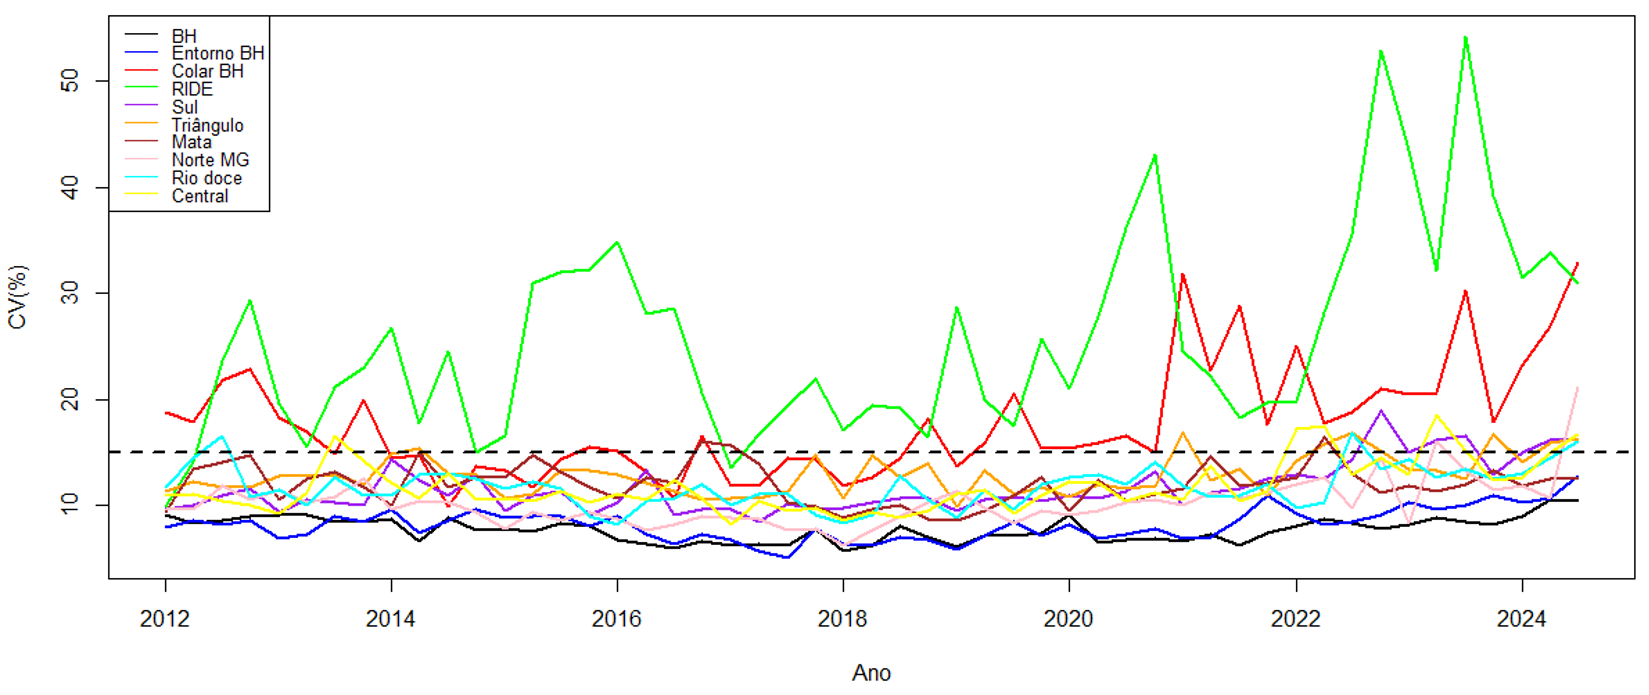
\includegraphics[width=1\linewidth]{Figs estratos/Coeficientes de variação - 10 estratos.png}
    \fonte{Elaboração própria, com base nos dados da PNAD Contínua. Nota: a linha pontilhada representa o valor de 15\%.}
    \label{fig:cvregs}
\end{figure}

\vspace{-1.5em}

A maior variabilidade das estimativas diretas está diretamente associada ao tamanho efetivo da amostra em cada estrato. Como mostra a Figura \ref{fig:amosdoms}, a RIDE de Brasília em Minas e o Colar Metropolitano de Belo Horizonte apresentam os menores contingentes de domicílios investigados ao longo do período. Na média da série analisada, essas regiões contaram, respectivamente, com aproximadamente 288 e 598 domicílios, valores bastante inferiores aos observados nos demais estratos.

\vspace{-1em}
\begin{figure}[H]
    \centering
    \caption{Evolução da amostra efetiva de domicílios -- dez estratos originais -- 1º trimestre de 2012 ao 4º trimestre de 2024}
    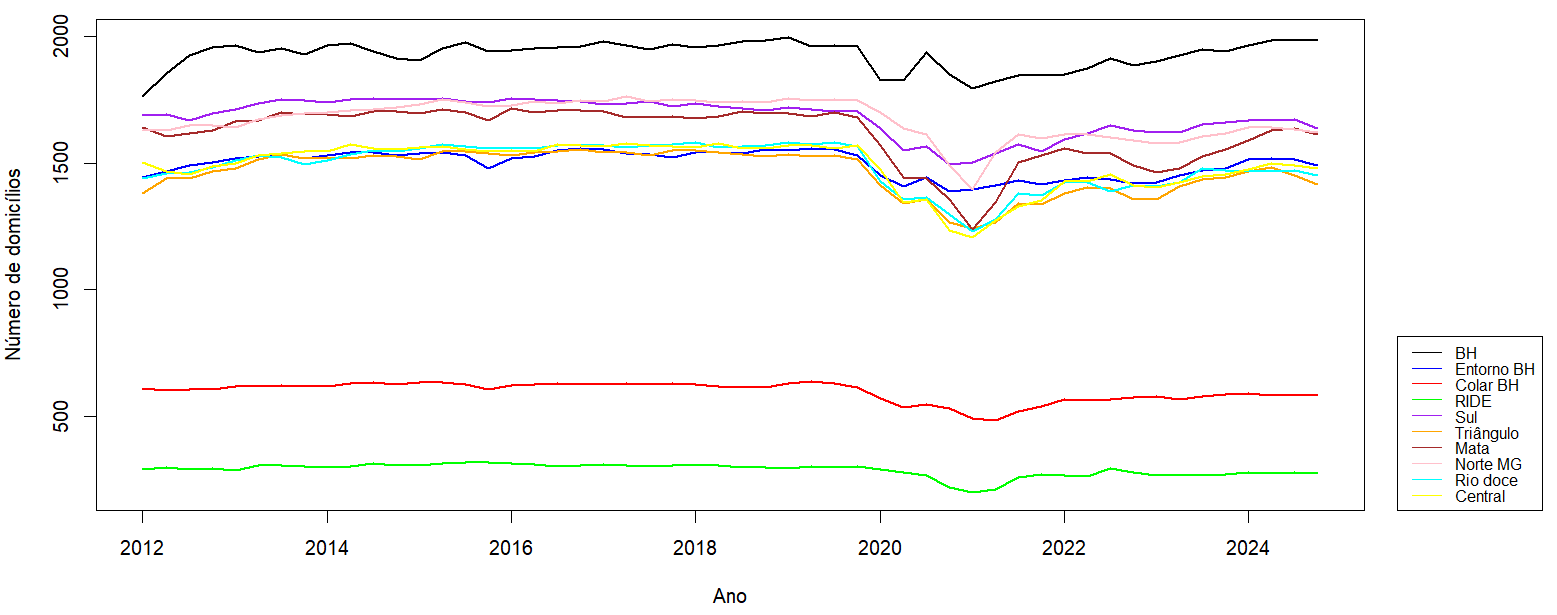
\includegraphics[width=1\linewidth]{Figs estratos/Amostra efetiva de domicílios - editado.png}
    \fonte{Elaboração própria, com base nos dados da PNAD Contínua.}
    \label{fig:amosdoms}
\end{figure}
\vspace{-1em}

A Tabela \ref{tab:cvmedest} sintetiza os coeficientes de variação médios das séries do total de desocupados e do total de ocupados para os oito estratos utilizados neste artigo, já considerando as agregações descritas anteriormente. Em geral, os coeficientes de variação são mais elevados para o total de desocupados do que para o total de ocupados, resultado esperado em razão do menor tamanho relativo da população desocupada. Belo Horizonte apresenta os menores coeficientes médios para ambas as variáveis. Já os estratos resultantes das agregações, Colar e Entorno Metropolitano de BH e Norte de Minas, passam a apresentar coeficientes médios inferiores a 15\%, reforçando a adequação da decisão metodológica adotada.

\vspace{-1em}
\begin{table}[H]
    \centering
    \captionsetup{justification=centering}
    \caption{Média do coeficiente de variação para os oito estratos geográficos de Minas Gerais -- 1º trimestre de 2012 ao 4º trimestre de 2024}
    \renewcommand{\arraystretch}{0.8}
    \resizebox{\textwidth}{!}{
    \begin{tabular}{@{}lcc@{}}
        \toprule
        \textbf{Estrato geográfico} & \textbf{Total de desocupados} & \textbf{Total de ocupados} \\
        \midrule
        01 -- Belo Horizonte & 7,9\% & 1,8\% \\
        02 -- Colar e Entorno Metropolitano de BH & 7,5\% & 2,1\% \\
        03 -- Sul de Minas & 11,8\% & 4,0\% \\
        04 -- Triângulo Mineiro & 13,0\% & 5,5\% \\
        05 -- Zona da Mata & 12,1\% & 4,5\% \\
        06 -- Norte de Minas & 10,2\% & 4,3\% \\
        07 -- Vale do Rio Doce & 11,9\% & 5,4\% \\
        08 -- Central & 11,9\% & 4,4\% \\
        \bottomrule
    \end{tabular}
    }
    \fonte{Elaboração própria, com base nos dados da PNAD Contínua.}
    \label{tab:cvmedest}
\end{table}
\vspace{-1em}

Portanto, a análise empírica deste artigo considera oito estratos geográficos para Minas Gerais. Essa opção preserva a capacidade de investigar diferenças regionais relevantes no interior do estado e, ao mesmo tempo, reduz a instabilidade das estimativas diretas nos domínios com menor tamanho amostral. A definição desses recortes é, assim, compatível com o objetivo do estudo: estimar tendências regionais do mercado de trabalho com maior precisão estatística, utilizando modelos estruturais aplicados a séries trimestrais da PNAD Contínua.

Essa opção deve ser entendida como uma escolha analítica voltada à produção de séries temporais regionais com precisão mínima para interpretação. Portanto, a agregação não elimina a heterogeneidade existente no interior dessas áreas, mas reduz a instabilidade amostral que comprometeria a leitura temporal dos menores estratos originais.

\section{Metodologia e base de dados}
\label{sec:metodologia}

A estratégia metodológica adotada neste artigo baseia-se em modelos estruturais de séries temporais na forma de espaço de estados, acrescidos de um componente explícito para o erro amostral. O objetivo é estimar as tendências das séries do total de desocupados, do total de ocupados e da taxa de desocupação nos oito estratos geográficos de Minas Gerais definidos na seção anterior. Para o total de desocupados e o total de ocupados, foram estimados modelos univariados e multivariados. A taxa de desocupação foi analisada por duas estratégias: estimação direta da própria taxa e cálculo indireto a partir das tendências estimadas para seus componentes.
\subsection{Modelo estrutural básico com erro amostral}
\label{subsec:meb}

A PNAD Contínua é uma pesquisa amostral repetida com sobreposição de amostra \citep{pnadNT}. Por essa razão, a aplicação de um modelo estrutural convencional, como em \citet{harvey1989}, deve ser complementada pela modelagem do erro amostral induzido pelo desenho da pesquisa. Seguindo a abordagem proposta por \citet{scott1974} e \citet{scott1977}, a estimativa direta observada no tempo \(t\), denotada por \(\hat{y}_t\), pode ser decomposta em dois componentes: o parâmetro populacional não observado \(\theta_t\), que representa o sinal de interesse, e o erro amostral \(e_t\):

\vspace{-0.5cm}
\begin{equation}
    \hat{y}_t = \theta_t + e_t.
    \label{eq:model}
\end{equation}

A Equação \ref{eq:model} define um modelo de extração de sinal. Nesse tipo de formulação, busca-se separar a evolução subjacente do indicador de interesse do ruído associado ao processo de amostragem. Em pesquisas amostrais repetidas, esse ruído pode apresentar dependência temporal, sobretudo quando há sobreposição de unidades amostrais entre períodos consecutivos. Por isso, o erro amostral não é tratado como ruído branco, mas modelado por processos autorregressivos ou de médias móveis, conforme indicado por \citet{scott1977}.

Como as variâncias do desenho amostral variam ao longo do tempo, adota-se a forma escalonada de \citet{binderdick1989}, em que o erro amostral é decomposto no produto entre o erro-padrão do desenho e um erro padronizado:

\vspace{-0.5cm}
\begin{equation}
    e_t = c_t\,\tilde{e}_t,
    \qquad c_t = \sqrt{V_{\text{des}}(\hat{y}_t)},
    \qquad V(\tilde{e}_t) = 1,
    \label{eq:erro_escalonado}
\end{equation}

\noindent
em que \(c_t\) é o erro-padrão publicado pelo IBGE para o período \(t\) e \(\tilde{e}_t\) segue o processo ARMA identificado. A restrição \(V(\tilde{e}_t)=1\) é imposta, e não estimada: sob ela, a variância marginal do erro amostral do modelo coincide, por construção, com a variância do desenho, e a variância da inovação do processo passa a ser \textit{derivada} dos coeficientes ARMA pela solução estacionária da equação de Lyapunov. Essa escolha tem consequência direta sobre a leitura dos resultados. Se \(V(\tilde{e}_t)\) fosse deixada livre, o modelo poderia reduzir o erro-padrão simplesmente atribuindo ao erro amostral variância inferior à do desenho, e o ganho de precisão medido confundir-se-ia com discordância em relação à variância publicada pelo IBGE. Sob a restrição, todo ganho reportado decorre da estrutura temporal e da dependência entre domínios, e não de uma reavaliação implícita do desenho amostral.

O processo do erro amostral foi identificado a partir das funções de autocorrelação (FAC) e autocorrelação parcial (FACP), calculadas para cada variável e estrato geográfico. Dada a restrição de acesso aos microdados completos da pesquisa, utilizou-se o método dos pseudo-erros, conforme \citet{silva2002}. Esse procedimento explora as diferenças entre estimativas produzidas para grupos de rotação da amostra e a estimativa agregada da série, de modo a aproximar o comportamento temporal do erro amostral. A Figura \ref{fig:facsul} ilustra, para o Sul de Minas, o processo de identificação a partir da FAC e da FACP.

A identificação foi conduzida \textit{individualmente} para cada uma das 24 combinações de estrato e indicador, e não por meio de uma especificação única imposta a todas as séries. Para cada combinação, os coeficientes de um conjunto de candidatos --- processos AR de ordem 1 a 4, MA de ordem 1 a 4 e ARMA(1,1) --- foram obtidos por casamento de momentos com a FAC estimada, e o modelo estrutural completo foi ajustado sob cada um deles. Entre os candidatos cujos resíduos padronizados não rejeitam a hipótese de brancura pelo teste de Ljung-Box a 5\%, selecionou-se o mais parcimonioso, com desempate pelo critério BIC.

Duas formulações foram excluídas do conjunto de candidatos por decisão metodológica. A primeira é o ruído branco: há autocorrelação detectável nos pseudo-erros em todas as séries, e adotá-lo equivaleria a abandonar a modelagem do erro amostral, que é justamente o objeto do procedimento. A segunda é o processo de médias móveis de ordem 4 implicado diretamente pelo esquema de rotação 1-2(5) da PNAD Contínua, cuja sobreposição amostral de \((5-j)/5\) impõe \(\theta_j = 1\) para \(j = 1, \ldots, 4\). Embora essa formulação seja teoricamente exata e branqueie bem os resíduos, a sobreposição que ela impõe mostrou-se sistematicamente mais forte do que a observada nos pseudo-erros, com o pior ajuste do conjunto de candidatos. A Tabela \ref{tab:modelos_arma} apresenta os processos assim selecionados.

\vspace{-0.2cm}
\begin{table}[!htb]
    \centering
    \captionsetup{justification=centering}
    \caption{Processo do erro amostral identificado por estrato geográfico e indicador}
    \resizebox{\textwidth}{!}{
    \begin{tabular}{@{}lccc@{}}
        \toprule
        \textbf{Estrato geográfico} & \textbf{Total de desocupados} & \textbf{Total de ocupados} & \textbf{Taxa de desocupação} \\
        \midrule
        01 -- Belo Horizonte & AR(1) & AR(1) & AR(1) \\
        02 -- Entorno e Colar Metropolitano de BH & MA(1) & AR(1) & MA(1) \\
        03 -- Sul de Minas & AR(1) & AR(1) & AR(1) \\
        04 -- Triângulo Mineiro & AR(1) & AR(1) & AR(1) \\
        05 -- Zona da Mata & AR(1) & AR(1) & AR(1) \\
        06 -- Norte de Minas & AR(1) & AR(1) & MA(1) \\
        07 -- Vale do Rio Doce & AR(1) & AR(1) & AR(1) \\
        08 -- Central & AR(3) & AR(1) & AR(3) \\
        \bottomrule
    \end{tabular}
    }
    \fonte{Elaboração própria, com base nos dados da PNAD Contínua. Nota: a identificação é individual por estrato e indicador. Entre os candidatos cujos resíduos não apresentam autocorrelação significativa pelo teste de Ljung-Box a 5\%, seleciona-se o mais parcimonioso, com desempate pelo BIC.}
    \label{tab:modelos_arma}
\end{table}

\vspace{-0.5cm}

\begin{figure}[!htb]
    \centering
     \caption{FAC e FACP calculadas para o Sul de Minas - total de ocupados}
    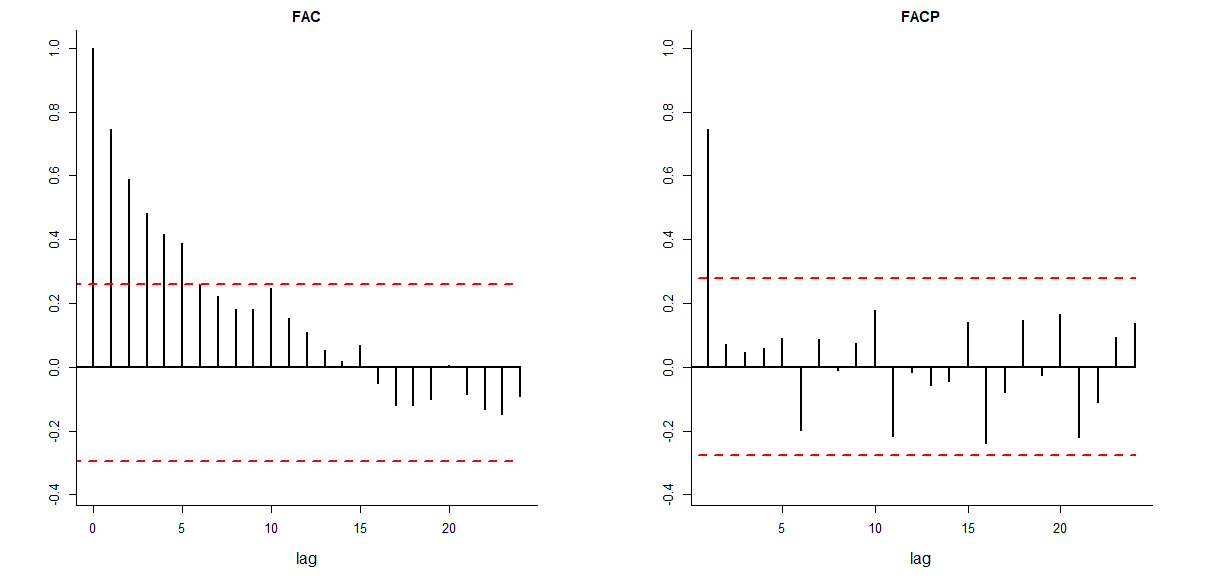
\includegraphics[width=1\linewidth, height=5.5cm]{Figs Metodologia/facsul.png}
    \fonte{Elaboração própria, com base nos dados da PNAD Contínua.}
    \label{fig:facsul}
\end{figure}

O parâmetro populacional não observado \(\theta_t\) foi especificado a partir do Modelo Estrutural Básico (MEB). Nesse modelo, \(\theta_t\) é decomposto em três componentes: tendência \(L_t\), sazonalidade \(S_t\) e componente irregular \(I_t\):

\begin{equation}
    \theta_t = L_t + S_t + I_t, 
    \quad I_t \sim \mathcal{N}(0,\sigma_I^2).
    \label{eq:decomposicao}
\end{equation}

A tendência é representada por um modelo de nível local com inclinação estocástica. Assim, o nível da série \(L_t\) evolui a partir do nível e da inclinação observados no período anterior, enquanto a inclinação \(R_t\) segue um passeio aleatório:

\vspace{-1cm}
\begin{equation}
    L_t = L_{t-1} + R_{t-1} + \eta_{L,t}, 
    \quad \eta_{L,t} \sim \mathcal{N}(0,\sigma_L^2),
    \label{eq:nivel}
\end{equation}
\vspace{-0.5cm}
\begin{equation}
    R_t = R_{t-1} + \eta_{R,t}, 
    \quad \eta_{R,t} \sim \mathcal{N}(0,\sigma_R^2).
    \label{eq:inclinacao}
\end{equation}

Assume-se que os distúrbios \(\eta_{L,t}\) e \(\eta_{R,t}\) são serialmente não correlacionados e mutuamente independentes. A sazonalidade foi especificada na forma trigonométrica, adequada para séries trimestrais, com \(s=4\):

\begin{equation}
    S_t = \sum_{l=1}^{s/2} S_{l,t},
    \label{eq:saztrig}
\end{equation}
\begin{equation}
\label{eq:sencos}
\begin{bmatrix}
S_{l,t} \\
S_{l,t}^{*}
\end{bmatrix}
=
\begin{bmatrix}
\cos(2\pi l/s) & \sin(2\pi l/s) \\
-\sin(2\pi l/s) & \cos(2\pi l/s)
\end{bmatrix}
\begin{bmatrix}
S_{l,t-1} \\
S_{l,t-1}^{*}
\end{bmatrix}
+
\begin{bmatrix}
\eta_{S,l,t} \\
\eta_{S,l,t}^{*}
\end{bmatrix}.
\end{equation}

\noindent 
Em que \(l = 1,2,\dots,\lfloor s/2 \rfloor\), e os distúrbios sazonais seguem \(\eta_{S,l,t} \sim WN(0,\sigma_S^2I)\), sendo não correlacionados entre diferentes frequências sazonais.

Além dos modelos univariados, foram estimados modelos multivariados para os três indicadores, considerando conjuntamente as séries dos oito estratos geográficos. Na formulação multivariada, os componentes \(L_t\), \(R_t\), \(S_t\), \(I_t\) e \(e_t\) passam a ser representados por vetores de dimensão \(P \times 1\), em que \(P=8\) corresponde ao número de estratos analisados. As variâncias dos distúrbios passam, portanto, a ser representadas por matrizes de covariância associadas aos respectivos componentes estruturais.

Foram considerados dois tipos de modelos multivariados. O primeiro, denominado modelo sem correlação entre os distúrbios das inclinações, estima conjuntamente as séries dos estratos, mas sem permitir dependência contemporânea entre os movimentos de tendência das diferentes regiões. O segundo, denominado modelo com correlação, permite que os distúrbios da inclinação da tendência sejam correlacionados entre os estratos geográficos. Essa especificação busca captar movimentos comuns na dinâmica regional do mercado de trabalho, explorando a possibilidade de ganho de precisão por meio do empréstimo de força entre domínios. A correlação entre os distúrbios das inclinações é dada por:

\vspace{-0.5cm}
\begin{equation}
\label{eq:covinclinacao}
    \mathrm{cov}(\eta_{R,y,p,t},\eta_{R,y,p',t}) =
    \rho^{R}_{y_p,y_{p'}}
    \sigma_{R,y_p}
    \sigma_{R,y_{p'}},
    \quad p \neq p',
\end{equation}

\noindent
em que \(p\) e \(p'\) indicam dois estratos geográficos distintos, e \(\rho^{R}_{y_p,y_{p'}}\) representa a correlação entre os distúrbios das inclinações das respectivas tendências.

A estimação dessa estrutura exige cuidado. Parametrizar diretamente os 28 coeficientes de correlação, restringindo cada um ao intervalo \((-1,1)\), garante que cada elemento seja individualmente admissível, mas não que o conjunto forme uma matriz de covariância válida --- isto é, positiva semidefinida. Com séries curtas e correlações elevadas, o otimizador pode convergir para configurações inadmissíveis, cujos coeficientes não admitem interpretação. Para evitar esse problema, adota-se aqui a parametrização por fator de Cholesky:

\vspace{-0.5cm}
\begin{equation}
    \Sigma_R = LL',
    \label{eq:cholesky}
\end{equation}

\noindent
em que \(L\) é triangular inferior com elementos diagonais positivos, obtidos por exponenciação dos parâmetros correspondentes. Sob essa formulação, qualquer valor dos \(P(P+1)/2 = 36\) parâmetros livres produz uma matriz \(\Sigma_R\) positiva semidefinida por construção, e a admissibilidade deixa de depender do resultado da otimização. Como a matriz estimada pode ter posto reduzido, reporta-se, junto com as correlações, o espectro de autovalores de \(\Sigma_R\), que indica quantas tendências comuns efetivamente sustentam a dependência entre os estratos.

A estimação foi realizada na forma de espaço de estados, utilizando o filtro de Kalman. De modo geral, um modelo em espaço de estados pode ser representado por uma equação de medida e uma equação de transição \citep{harvey1989,durbinkoop2012}:

\vspace{-0.5cm}
\begin{equation}
    y_t = c_t + Z_t\alpha_t + \varepsilon_t,
    \label{eq:medida}
\end{equation}
\vspace{-0.8cm}
\begin{equation}
    \alpha_{t+1} = d_t + T_t\alpha_t + v_t.
    \label{eq:transicao}
\end{equation}

\noindent
Na Equação \ref{eq:medida}, \(y_t\) representa o vetor de observações, \(\alpha_t\) é o vetor de estados, \(Z_t\) é a matriz que relaciona os estados às observações, \(c_t\) é um vetor de constantes e \(\varepsilon_t\) é o distúrbio da equação de medida, com média zero e matriz de covariância \(H_t\). Na Equação \ref{eq:transicao}, \(T_t\) é a matriz de transição dos estados, \(d_t\) é um vetor de constantes e \(v_t\) é o distúrbio da equação de transição, com média zero e matriz de covariância \(Q_t\). O filtro de Kalman permite estimar recursivamente os estados não observados e, posteriormente, obter as estimativas suavizadas dos componentes de interesse.

Os diagnósticos dos modelos foram realizados com base nos resíduos padronizados. Foram aplicados o teste de Shapiro-Wilk para avaliar a normalidade dos resíduos \citep{shapiro_wilk_1965}, o teste \(H\) para avaliar a presença de heterocedasticidade \citep{durbinkoop2012} e o teste de Ljung-Box para verificar autocorrelação serial remanescente \citep{ljung_box_1978}. A comparação entre as especificações univariada e multivariada baseia-se na diferença relativa média do erro-padrão e no vício relativo em relação às estimativas diretas, complementadas pela análise da estrutura da matriz de covariância dos distúrbios das inclinações \citep{durbinkoop2012,pelagatti2016}.

\subsection{Base de dados}
\label{subsec:base}

As séries utilizadas correspondem ao total de desocupados, ao total de ocupados e à taxa de desocupação da PNAD Contínua para os estratos geográficos de Minas Gerais. Foram consideradas séries trimestrais do primeiro trimestre de 2012 ao quarto trimestre de 2024, totalizando 52 observações para cada indicador e estrato geográfico \citep{ibge2025pnad}.

Para os oito estratos analisados, foram organizadas séries das estimativas diretas, dos respectivos erros-padrão e dos coeficientes de variação. Também foram coletadas estimativas por grupo de rotação da amostra, necessárias para a construção dos pseudo-erros utilizados na identificação do processo do erro amostral. No total, a base principal reúne 24 séries trimestrais: oito séries do total de desocupados, oito séries do total de ocupados e oito séries da taxa de desocupação.

O banco de dados foi construído no \textit{software} R \citep{R-base}, com o apoio dos pacotes \textit{PNADcIBGE} \citep{pacotepnad} e \textit{survey} \citep{survey}. Os modelos estruturais foram estimados no R por meio do pacote \textit{dlm} \citep{dlm}.

\section{Resultados}
\label{sec:resultados}

Esta seção apresenta os resultados da estimação das tendências do total de desocupados, do total de ocupados e da taxa de desocupação para os oito estratos geográficos de Minas Gerais. As séries foram modeladas por meio do Modelo Estrutural Básico com incorporação explícita do erro amostral, estimado na forma de espaço de estados pelo filtro de Kalman.

As subseções seguintes discutem, para cada indicador, os hiperparâmetros estimados, os diagnósticos dos resíduos, as medidas de desempenho em relação às estimativas diretas e a evolução temporal das tendências estimadas.

\subsection{Total de desocupados}

A Tabela \ref{tab:hiperdesoc} apresenta os hiperparâmetros estimados para os componentes do modelo aplicado ao total de desocupados, bem como o processo do erro amostral identificado individualmente em cada estrato. O hiperparâmetro associado à sazonalidade assumiu comportamento determinístico em todos os estratos, inclusive no modelo multivariado. A variância da inovação do erro amostral, \(\hat{\sigma}_{\tilde{e}}^2\), situou-se entre 0,69 e 0,95; convém lembrar que ela não é estimada, mas derivada dos coeficientes do processo pela restrição \(V(\tilde{e}_t)=1\), de modo que coincide nos dois modelos.

O componente irregular foi estimado em valor praticamente nulo em todos os estratos. Esse resultado não deve ser lido como ausência de choques transitórios, e sim como reflexo da fraca identificação do componente: o perfil de verossimilhança é quase plano em \(\sigma_I^2\), de modo que variar essa variância entre 0,1\% e 10\% da variância do desenho altera a log-verossimilhança em menos de 0,3, contra o limiar de 1,92 de um teste a 5\%. Uma consequência prática relevante é que, com \(\hat{\sigma}_I^2 \approx 0\), o irregular obtido por diferença é nulo e a série dessazonalizada coincide com a tendência estimada. A separação entre tendência e choques transitórios, portanto, não é sustentada pelos dados nesta especificação, e este artigo não a reivindica.

\vspace{-0.3cm}
\begin{table}[H]
\centering
\captionsetup{justification=centering}
\caption{Hiperparâmetros estimados para o total de desocupados - modelos univariado e multivariado}
\label{tab:hiperdesoc}
\scalebox{0.92}{
\renewcommand{\arraystretch}{0.85}
\begin{tabular}{llccccc}
\toprule
& & \multicolumn{5}{c}{\textbf{Modelo Univariado}} \\
\cmidrule(lr){3-7}
\textbf{Estrato geográfico} & \textbf{Processo} & \(\hat{\sigma}_L^2\) & \(\hat{\sigma}_R^2\) & \(\hat{\sigma}_S^2\) & \(\hat{\sigma}_I^2\) & \(\hat{\sigma}_{\tilde{e}}^2\) \\
\midrule
01 - Belo Horizonte & AR(1) & 0,0483 & 18,4914 & 0,0000 & 0,0000 & 0,9052 \\
02 - Entorno e Colar Metropolitano de BH & MA(1) & 0,0161 & 102,7494 & 0,0000 & 0,0000 & 0,8524 \\
03 - Sul de Minas & AR(1) & 82,4451 & 1,1848 & 0,0000 & 0,0000 & 0,8467 \\
04 - Triângulo Mineiro & AR(1) & 0,0246 & 8,3891 & 0,0000 & 0,0000 & 0,9517 \\
05 - Zona da Mata & AR(1) & 46,8067 & 0,5211 & 0,0000 & 0,0000 & 0,9046 \\
06 - Norte de Minas & AR(1) & 127,4207 & 1,4080 & 0,0000 & 0,0000 & 0,7976 \\
07 - Vale do Rio Doce & AR(1) & 112,0160 & 1,1011 & 0,0000 & 0,0000 & 0,6863 \\
08 - Central & AR(3) & 0,0306 & 21,8547 & 0,0000 & 0,0000 & 0,9062 \\
\midrule
& & \multicolumn{5}{c}{\textbf{Modelo Multivariado}} \\
\cmidrule(lr){3-7}
\textbf{Estrato geográfico} & \textbf{Processo} & \(\hat{\sigma}_L^2\) & \(\hat{\sigma}_R^2\) & \(\hat{\sigma}_S^2\) & \(\hat{\sigma}_I^2\) & \(\hat{\sigma}_{\tilde{e}}^2\) \\
\midrule
01 - Belo Horizonte & AR(1) & 0,0239 & 33,8915 & 0,0000 & 0,0000 & 0,9052 \\
02 - Entorno e Colar Metropolitano de BH & MA(1) & 0,0060 & 112,5743 & 0,0000 & 0,0000 & 0,8524 \\
03 - Sul de Minas & AR(1) & 0,0658 & 19,8207 & 0,0000 & 0,0000 & 0,8467 \\
04 - Triângulo Mineiro & AR(1) & 0,0383 & 13,5033 & 0,0000 & 0,0000 & 0,9517 \\
05 - Zona da Mata & AR(1) & 1,1664 & 10,7285 & 0,0000 & 0,0000 & 0,9046 \\
06 - Norte de Minas & AR(1) & 0,5315 & 27,4822 & 0,0000 & 0,0000 & 0,7976 \\
07 - Vale do Rio Doce & AR(1) & 0,7853 & 30,7076 & 0,0000 & 0,0000 & 0,6863 \\
08 - Central & AR(3) & 0,0474 & 15,3830 & 0,0000 & 0,0000 & 0,9062 \\
\bottomrule
\end{tabular}}
\fonte{Elaboração própria, com base nos dados da PNAD Contínua. Nota: o processo do erro amostral é identificado individualmente por estrato (Seção \ref{sec:metodologia}), e \(\hat{\sigma}_{\tilde{e}}^2\) é derivada dos coeficientes do processo, por isso coincidindo nos dois modelos. Sobre \(\sigma_I^2\), ver a ressalva de identificação no texto.}
\end{table}

\vspace{-0.7cm}

A escolha dos valores iniciais dos hiperparâmetros foi realizada a partir de um procedimento exploratório. Inicialmente, estimou-se um Modelo Estrutural Básico sem erro amostral, cujos resultados serviram como referência para a definição de quatro valores iniciais alternativos para cada parâmetro. Em seguida, o Modelo Estrutural Básico com erro amostral foi estimado para cada combinação de valores iniciais, sendo selecionada a especificação com melhor valor da função de verossimilhança, isto é, maior log-verossimilhança ou, quando a implementação retorna a log-verossimilhança negativa, menor valor da função objetivo.\footnote{Para os parâmetros de correlação do modelo multivariado, os valores iniciais foram fixados em zero.}

Esse procedimento foi inicialmente aplicado aos modelos univariados e, posteriormente, os valores selecionados foram utilizados como referência para a estimação dos modelos multivariados. A estratégia contribuiu para a obtenção de modelos mais estáveis, tanto em termos dos hiperparâmetros estimados quanto dos diagnósticos dos resíduos.

A Tabela \ref{tab:diagdesoc} apresenta os testes de diagnóstico dos resíduos. Considerando o nível de significância de 5\%, os resíduos do modelo univariado não rejeitaram nenhuma das três hipóteses em nenhum dos estratos. No modelo multivariado, registram-se duas rejeições isoladas: a normalidade no Vale do Rio Doce (\(p=0{,}040\)) e a ausência de autocorrelação no Norte de Minas (\(p=0{,}001\)); não há evidência de heterocedasticidade em nenhum estrato. Embora a normalidade dos resíduos seja uma condição desejável, \citet{harvey1989} ressalta que, mesmo sob desvios dessa hipótese, o estimador obtido pelo filtro de Kalman preserva propriedades ótimas no sentido de minimizar o erro quadrático médio, desde que a especificação linear seja mantida.

\vspace{-0.3cm}
\begin{table}[H]
\centering
\captionsetup{justification=centering}
\caption{Teste de diagnóstico do resíduo para o total de desocupados - modelos univariado e multivariado}
\label{tab:diagdesoc}
\scalebox{1}{
\renewcommand{\arraystretch}{0.7}
\begin{tabular}{lccc}
\toprule
& \multicolumn{3}{c}{\textbf{Modelo Univariado}} \\
\cmidrule(lr){2-4}
\textbf{Estrato geográfico} & Shapiro-Wilk & Ljung-Box & H \\
\midrule
01 - Belo Horizonte & 0,9769 & 0,6518 & 0,6333 \\
02 - Entorno e Colar Metropolitano de BH & 0,4622 & 0,0530* & 0,7115 \\
03 - Sul de Minas & 0,0917* & 0,0607* & 0,8793 \\
04 - Triângulo Mineiro & 0,0539* & 0,4577 & 0,9610 \\
05 - Zona da Mata & 0,6087 & 0,2385 & 0,6497 \\
06 - Norte de Minas & 0,7141 & 0,0848* & 0,7214 \\
07 - Vale do Rio Doce & 0,9441 & 0,8272 & 0,0997* \\
08 - Central & 0,7268 & 0,0928* & 0,1300 \\
\midrule
& \multicolumn{3}{c}{\textbf{Modelo Multivariado}} \\
\cmidrule(lr){2-4}
\textbf{Estrato geográfico} & Shapiro-Wilk & Ljung-Box & H \\
\midrule
01 - Belo Horizonte & 0,7846 & 0,1710 & 0,3265 \\
02 - Entorno e Colar Metropolitano de BH & 0,6429 & 0,0684* & 0,7184 \\
03 - Sul de Minas & 0,1143 & 0,0743* & 0,7924 \\
04 - Triângulo Mineiro & 0,7553 & 0,2309 & 0,3836 \\
05 - Zona da Mata & 0,1534 & 0,2716 & 0,8799 \\
06 - Norte de Minas & 0,3554 & 0,0010*** & 0,2680 \\
07 - Vale do Rio Doce & 0,0404** & 0,3737 & 0,1733 \\
08 - Central & 0,7102 & 0,7748 & 0,6216 \\
\bottomrule
\end{tabular}}
\fonte{Elaboração própria, com base nos dados da PNAD Contínua. Nota: * representa rejeição de \(H_0\) a 10\%, ** a 5\% e *** a 1\%. As oito primeiras observações foram descartadas, em razão do período de estabilização do filtro de Kalman.}
\end{table}

\vspace{-0.3cm}

A diferença observada entre os diagnósticos dos modelos univariado e multivariado levanta a questão sobre a contribuição das correlações incorporadas ao modelo multivariado. Conforme \citet{durbinkoop2012}, o modelo de equações de séries temporais aparentemente não correlacionadas, ou \textit{seemingly unrelated time series equations}, permite que séries modeladas de forma semelhante apresentem correlação entre os distúrbios de seus componentes. Sem a incorporação dessas correlações, os resultados do modelo multivariado tendem a se aproximar dos resultados dos modelos univariados. Por essa razão, é possível testar se os parâmetros adicionais de correlação são estatisticamente diferentes de zero.

A Tabela \ref{tab:matriz_correlacao_desoc} apresenta as correlações estimadas entre os distúrbios das inclinações. A matriz de covariância desses distúrbios é parametrizada por um fator de Cholesky, \(\Sigma_R = LL'\), o que garante que a estimativa seja positiva semidefinida por construção. Essa escolha é relevante porque a estimação livre das correlações duas a duas restringe cada coeficiente ao intervalo \((-1,1)\), mas não assegura que o conjunto das estimativas constitua uma matriz de covariância admissível.

Os coeficientes estimados situam-se, em geral, acima de 0,93, e a decomposição espectral da matriz revela apenas dois autovalores relevantes (254,77 e 8,86, contra 0,34; 0,12 e quatro valores inferiores a \(10^{-3}\)). Esse padrão indica que as oito séries compartilham um número muito reduzido de tendências comuns, e não que existam oito trajetórias regionais cujas correlações possam ser interpretadas isoladamente. Com 52 observações trimestrais, os 28 parâmetros de correlação não são identificados individualmente, e a leitura adequada da tabela é a de uma estrutura de posto reduzido.

Nesse contexto, o resultado regional que se destaca é o da Zona da Mata, único estrato cujas correlações com os demais permanecem em patamar substancialmente inferior, entre 0,54 e 0,69. A trajetória da tendência do total de desocupados nessa região acompanha apenas parcialmente o movimento comum aos demais estratos mineiros.

\vspace{-0.3cm}
\begin{table}[H]
\centering
\captionsetup{justification=centering}
\caption{Correlação estimada entre os distúrbios das inclinações - modelo multivariado - total de desocupados}
\label{tab:matriz_correlacao_desoc}

\renewcommand{\arraystretch}{0.8}

\resizebox{\linewidth}{!}{%
\begin{tabular}{@{}p{2.8cm}c*{8}{c}@{}}
\toprule
\textbf{Estrato Geográfico} & \(\hat{\sigma}_R^2\) & \textbf{1} & \textbf{2} & \textbf{3} & \textbf{4} & \textbf{5} & \textbf{6} & \textbf{7} & \textbf{8} \\
\midrule
01 - Belo Horizonte & 33,8915 & 1 &  &  &  &  &  &  &  \\
\raisebox{0em}{\parbox[t]{2.8cm}{02 - Entorno e Colar \\[-2pt] Metropolitano de BH}} & 112,5743 & 0,9911 & 1 &  &  &  &  &  &  \\
03 - Sul de Minas & 19,8207 & 0,9801 & 0,9910 & 1 &  &  &  &  &  \\
04 - Triângulo Mineiro & 13,5033 & 0,9879 & 0,9977 & 0,9978 & 1 &  &  &  &  \\
05 - Zona da Mata & 10,7285 & 0,5403 & 0,6164 & 0,6914 & 0,6554 & 1 &  &  &  \\
06 - Norte de Minas & 27,4822 & 0,9800 & 0,9930 & 0,9997 & 0,9986 & 0,6916 & 1 &  &  \\
07 - Vale do Rio Doce & 30,7076 & 0,9527 & 0,9797 & 0,9923 & 0,9882 & 0,7555 & 0,9937 & 1 &  \\
08 - Central & 15,3830 & 0,9894 & 0,9762 & 0,9503 & 0,9654 & 0,4365 & 0,9513 & 0,9181 & 1 \\
\bottomrule
\end{tabular}%
}

\fonte{Elaboração própria, com base nos dados da PNAD Contínua. Nota: autovalores estimados de \(\Sigma_R\): 254,769; 8,858; 0,343; 0,120 e 4 valores inferiores a \(10^{-3}\). Posto numérico de 7 em 8; posto \textbf{efetivo} de 2, contando os autovalores que retêm ao menos 1\% do maior. As correlações devem, portanto, ser lidas em conjunto, e não isoladamente.}
\end{table}

\vspace{-0.4cm}

O desempenho dos modelos foi avaliado por meio de duas medidas: a diferença relativa média do erro-padrão e o vício relativo médio. A primeira mede a redução percentual do erro-padrão da estimativa baseada em modelo em relação à estimativa direta, indicando ganho de precisão. A segunda avalia o afastamento médio do sinal estimado em relação à estimativa direta. Os resultados são apresentados na Tabela \ref{tab:diffviciodesoc}.

\vspace{-0.3cm}
\begin{table}[H]
\centering
\captionsetup{justification=centering}
\caption{Medidas de desempenho dos modelos univariado e multivariado - total de desocupados}
\label{tab:diffviciodesoc}
{%
\renewcommand{\arraystretch}{0.8}
\scalebox{0.95}{%
\begin{tabular}{lcccc}
\toprule
& \multicolumn{2}{c}{\textbf{\makecell{Diferença relativa média \\ do erro padrão (\%)}}} & \multicolumn{2}{c}{\textbf{Vício relativo (\%)}} \\
\cmidrule(lr){2-3} \cmidrule(lr){4-5}
\multicolumn{1}{l}{\textbf{Estrato Geográfico}} & \textbf{Univariado} & \textbf{Multivariado} & \textbf{Univariado} & \textbf{Multivariado} \\
\midrule
01 - Belo Horizonte & 11,87 & 29,03 & -0,16 & 0,37 \\
02 - Entorno e Colar Metropolitano de BH & 6,85 & 26,42 & 0,19 & 1,29 \\
03 - Sul de Minas & 11,70 & 37,17 & -1,27 & -3,16 \\
04 - Triângulo Mineiro & 21,75 & 50,11 & -1,03 & -2,58 \\
05 - Zona da Mata & 16,86 & 20,48 & -1,41 & -1,02 \\
06 - Norte de Minas & 9,13 & 35,70 & -0,57 & -1,62 \\
07 - Vale do Rio Doce & 6,15 & 25,04 & -1,37 & -3,69 \\
08 - Central & 11,67 & 37,56 & -0,85 & -3,48 \\
\midrule
\textbf{Média} & \textbf{12,00} & \textbf{32,69} & & \\
\bottomrule
\end{tabular}%
}
}
\fonte{Elaboração própria, com base nos dados da PNAD Contínua. Nota: as oito primeiras observações de cada série foram descartadas do cálculo, em razão do período de estabilização do filtro de Kalman.}
\end{table}

\vspace{-0.4cm}

Em relação à diferença relativa média do erro-padrão, ambos os modelos apresentaram ganhos em todos os estratos, evidenciando melhora de precisão em relação às estimativas diretas. O ganho médio foi de 12,0\% na especificação univariada e de 32,7\% na multivariada. O modelo multivariado apresentou desempenho superior em todos os oito estratos, com destaque para o Triângulo Mineiro (50,1\%), a região Central (37,6\%) e o Sul de Minas (37,2\%). O menor ganho da especificação multivariada ocorreu na Zona da Mata (20,5\%), justamente o estrato menos correlacionado com os demais.

Quanto ao vício relativo, os resultados indicam proximidade entre as estimativas baseadas em modelo e as estimativas diretas, com afastamento médio inferior a 4\% em todos os estratos nos dois modelos. O modelo univariado apresentou vício menor em sete dos oito estratos, o que é esperado: quanto mais o modelo suaviza, maior o ganho de precisão e maior o afastamento em relação à estimativa direta. O contraste entre as duas colunas expressa esse compromisso, e não uma falha de especificação.

As Figuras \ref{fig:est_desoc_1} e \ref{fig:est_desoc_2} apresentam as tendências estimadas para o total de desocupados e seus respectivos coeficientes de variação ao longo do período analisado.

Para o total de desocupados, o sinal estimado permaneceu dentro dos intervalos de confiança de 95\% das estimativas diretas em 348 dos 352 pontos analisados, ou seja, em 98,9\% dos casos. As trajetórias dos modelos se diferenciaram de forma mais perceptível no Sul de Minas, no Triângulo Mineiro e no Norte de Minas, estratos em que o modelo multivariado produziu tendências mais suavizadas.

Em termos de precisão, todas as regiões apresentaram redução dos coeficientes de variação em relação às estimativas diretas. Em nenhum ponto da série os coeficientes de variação das estimativas baseadas no modelo multivariado ultrapassaram 15\%, com máximo de 14,0\% no Vale do Rio Doce. Esse resultado reforça a capacidade dos modelos estruturais de filtrar a variabilidade associada ao erro amostral, recuperando uma trajetória mais estável do parâmetro populacional.

Na comparação entre especificações, o modelo multivariado apresentou coeficiente de variação médio menor que o univariado nos oito estratos. O contraste mais expressivo ocorre no Triângulo Mineiro, região em que a estimativa direta apresenta coeficiente de variação médio de 13,1\% e o modelo multivariado o reduz para 6,6\%. Em Belo Horizonte, a redução vai de 7,7\% para 5,4\%.

Diante do conjunto de evidências, considera-se que o modelo multivariado apresentou desempenho superior para o total de desocupados, sobretudo em relação à precisão das estimativas. O ganho é coerente com a estrutura de dependência estimada: como a matriz de covariância dos distúrbios das inclinações tem posto efetivo dois, há forte tendência comum entre os estratos, e é justamente essa dependência que a especificação multivariada explora ao tomar emprestada informação entre domínios.

\clearpage
\begin{figure}[H]
    \centering
    \caption{Estimativas da tendência para o total de desocupados e respectivos coeficientes de variação -- regiões 1 a 4 -- 1º trimestre de 2014 ao 4º trimestre de 2024}
    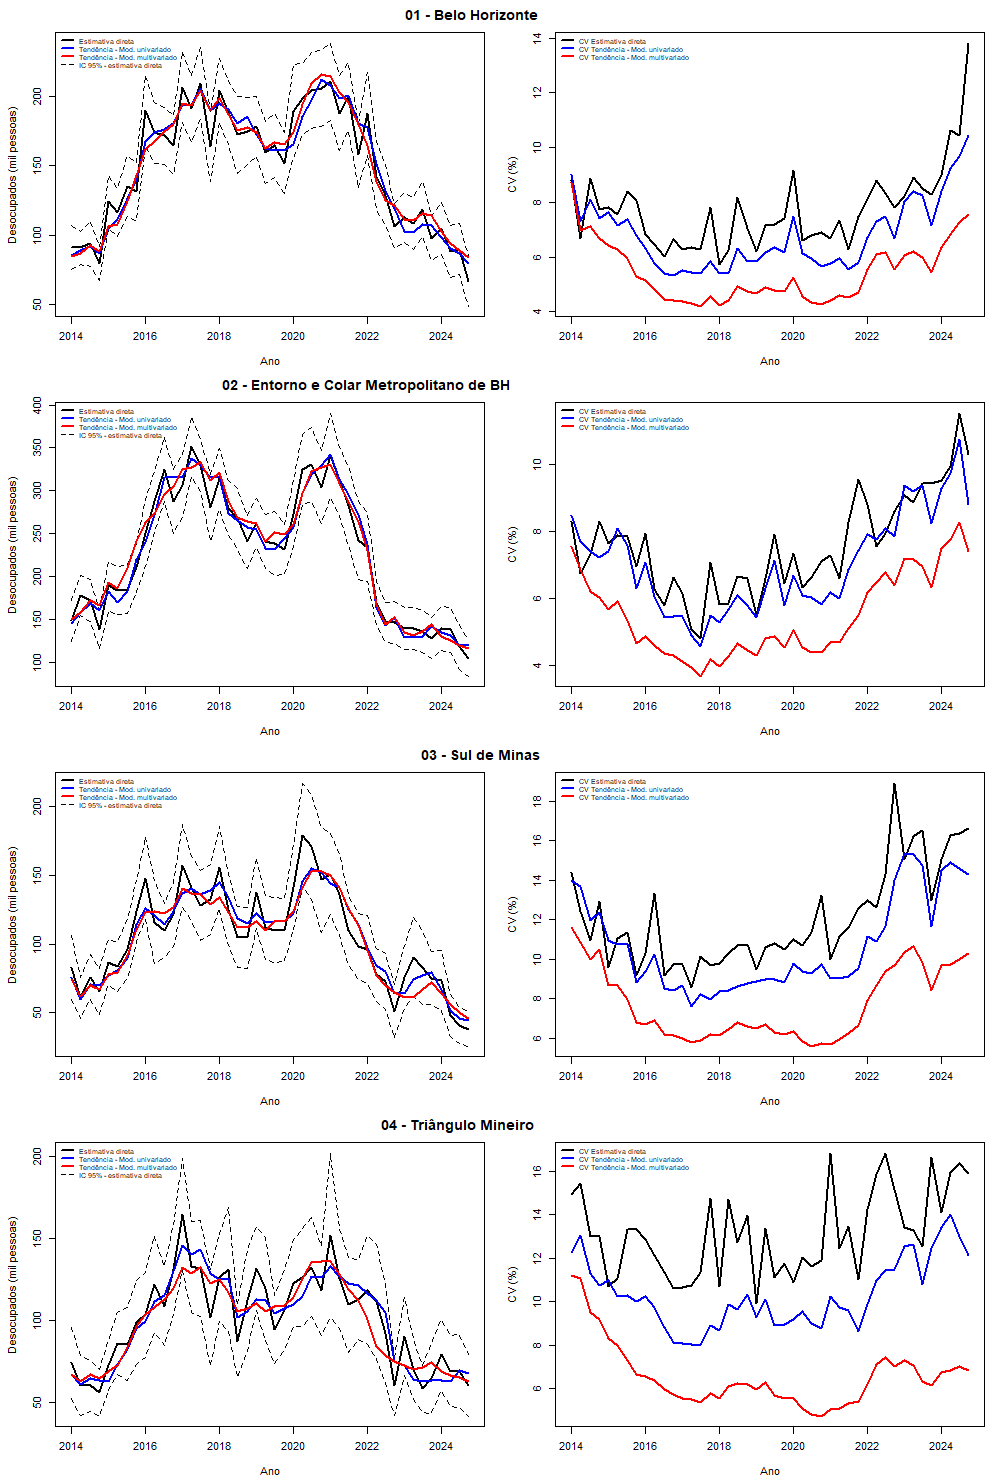
\includegraphics[width=0.85\linewidth]{resultados/Total de desocupados/Figura_Desocupacao_1.png}
    \fonte{Elaboração própria, com base nos dados da PNAD Contínua.}
    \label{fig:est_desoc_1}
\end{figure}

\begin{figure}[H]
    \centering
    \caption{Estimativas da tendência para o total de desocupados e respectivos coeficientes de variação -- regiões 5 a 8 -- 1º trimestre de 2014 ao 4º trimestre de 2024}
    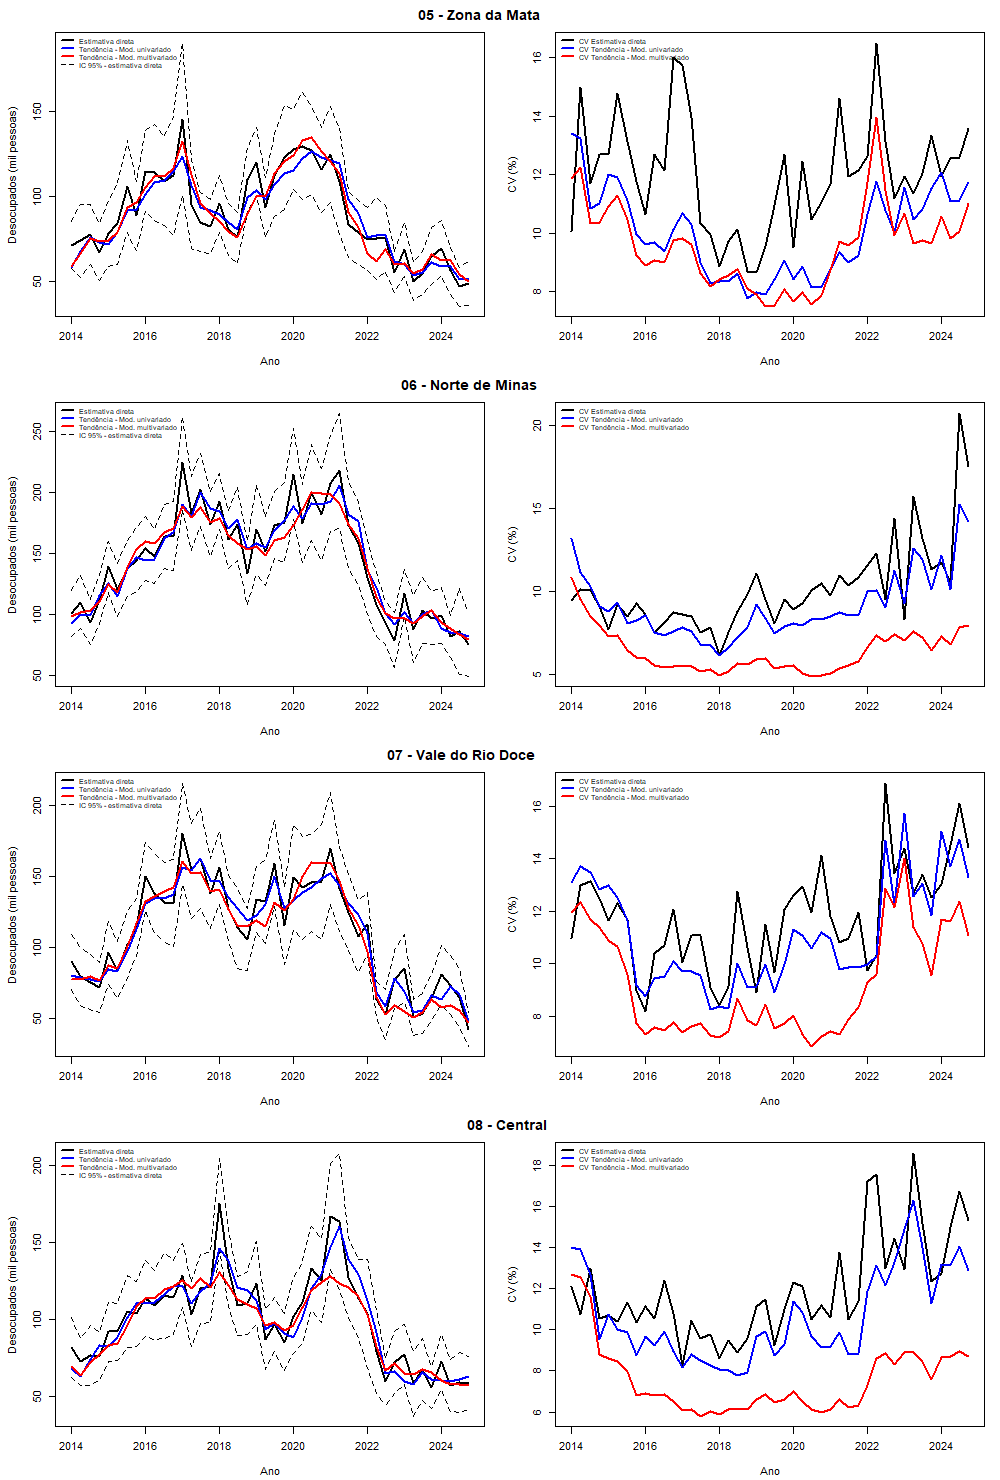
\includegraphics[width=0.85\linewidth]{resultados/Total de desocupados/Figura_Desocupacao_2.png}
    \fonte{Elaboração própria, com base nos dados da PNAD Contínua.}
    \label{fig:est_desoc_2}
\end{figure}



A Tabela \ref{tab:pontual_desoc} apresenta as estimativas pontuais do modelo multivariado para o último trimestre da série e as compara com as estimativas diretas do mesmo período.

\vspace{-1cm}
\begin{table}[H]
\centering
\captionsetup{justification=centering}
\caption{Resultados pontuais do modelo multivariado para o total de desocupados - 4\textordmasculine{} trimestre de 2024}
\label{tab:pontual_desoc}

\renewcommand{\arraystretch}{0.8}
\resizebox{\linewidth}{!}{%
\begin{tabular}{@{}p{2.8cm}cccccc@{}}
\toprule
\textbf{Estrato Geográfico} & $\hat{y}$ & $CV(\hat{y})$ & IC 95\% & $\hat{\theta}$ & $CV(\hat{\theta})$ & IC 95\% \\
\midrule
01 - Belo Horizonte & 67,03 & 13,81\% & [48,89 ; 85,18] & 72,34 & 8,84\% & [59,81 ; 84,87] \\
\raisebox{0em}{\parbox[t]{2.8cm}{02 - Entorno e Colar \\[-2pt] Metropolitano de BH}} & 104,59 & 10,29\% & [83,49 ; 125,69] & 100,09 & 8,48\% & [83,46 ; 116,73] \\
03 - Sul de Minas & 38,33 & 16,65\% & [25,82 ; 50,84] & 39,90 & 11,88\% & [30,61 ; 49,18] \\
04 - Triângulo Mineiro & 60,54 & 15,89\% & [41,69 ; 79,40] & 55,94 & 8,37\% & [46,77 ; 65,12] \\
05 - Zona da Mata & 48,48 & 13,59\% & [35,57 ; 61,39] & 47,49 & 11,56\% & [36,73 ; 58,24] \\
06 - Norte de Minas & 75,76 & 17,56\% & [49,69 ; 101,83] & 71,78 & 9,28\% & [58,73 ; 84,83] \\
07 - Vale do Rio Doce & 42,51 & 14,42\% & [30,49 ; 54,53] & 41,62 & 12,33\% & [31,56 ; 51,67] \\
08 - Central & 58,28 & 15,33\% & [40,77 ; 75,79] & 51,37 & 10,02\% & [41,29 ; 61,46] \\
\bottomrule
\end{tabular}%
}
\fonte{Elaboração própria, com base nos dados da PNAD Contínua. Nota: \(\hat{y}\) é a estimativa direta e \(\hat{\theta}\) o sinal estimado pelo modelo multivariado (tendência mais sazonalidade). Valores em milhares de pessoas.}
\end{table}

\vspace{-1cm}

No contexto posterior à crise sanitária da Covid-19, observou-se redução da precisão das estimativas diretas. Mesmo após o período mais agudo da pandemia, os coeficientes de variação de alguns estratos permaneceram elevados e não retornaram aos níveis observados antes da crise. Em contrapartida, os coeficientes de variação das estimativas baseadas no modelo multivariado permaneceram abaixo de 15\% em todos os estratos e em todo o período, resultando em intervalos de confiança mais estreitos.

\subsection{Total de ocupados}

A Tabela \ref{tab:hiperocup} apresenta os hiperparâmetros estimados para o total de ocupados. Diferentemente do observado para o total de desocupados, a identificação do erro amostral selecionou o mesmo processo, AR(1), em todos os oito estratos. Os modelos univariado e multivariado produziram estimativas muito próximas para os hiperparâmetros da tendência, com diferença perceptível apenas em \(\hat{\sigma}_R^2\) no Triângulo Mineiro e no Vale do Rio Doce.

A sazonalidade manteve comportamento determinístico em ambos os modelos e em todos os estratos. O componente irregular, tal como no total de desocupados, foi estimado em valor praticamente nulo, com a mesma ressalva de fraca identificação registrada anteriormente. Cabe notar que essa ressalva vale também para \(\sigma_S^2\): o caráter determinístico da sazonalidade não é, na maior parte dos casos, uma conclusão dos dados, mas o reflexo de um perfil de verossimilhança plano. A variância da inovação do erro amostral situou-se entre 0,39 e 0,58, refletindo apenas os coeficientes autorregressivos identificados, uma vez que é derivada da restrição \(V(\tilde{e}_t)=1\).

\vspace{-0.3cm}
\begin{table}[H]
\centering
\captionsetup{justification=centering}
\caption{Hiperparâmetros estimados para o total de ocupados - modelos univariado e multivariado}
\label{tab:hiperocup}
\scalebox{0.92}{
\renewcommand{\arraystretch}{0.85}
\begin{tabular}{llccccc}
\toprule
& & \multicolumn{5}{c}{\textbf{Modelo Univariado}} \\
\cmidrule(lr){3-7}
\textbf{Estrato geográfico} & \textbf{Processo} & \(\hat{\sigma}_L^2\) & \(\hat{\sigma}_R^2\) & \(\hat{\sigma}_S^2\) & \(\hat{\sigma}_I^2\) & \(\hat{\sigma}_{\tilde{e}}^2\) \\
\midrule
01 - Belo Horizonte & AR(1) & 429,6609 & 0,8061 & 0,0000 & 0,0000 & 0,5640 \\
02 - Entorno e Colar Metropolitano de BH & AR(1) & 826,3711 & 6,7883 & 0,0000 & 0,0000 & 0,5534 \\
03 - Sul de Minas & AR(1) & 0,3494 & 4,4507 & 0,0000 & 0,0000 & 0,4652 \\
04 - Triângulo Mineiro & AR(1) & 7,8799 & 7,8544 & 0,0000 & 0,0000 & 0,3975 \\
05 - Zona da Mata & AR(1) & 5,1703 & 10,4187 & 0,0000 & 0,0000 & 0,5184 \\
06 - Norte de Minas & AR(1) & 607,6945 & 2,3814 & 0,0000 & 0,0023 & 0,5275 \\
07 - Vale do Rio Doce & AR(1) & 0,0000 & 0,0005 & 0,0022 & 0,0001 & 0,3867 \\
08 - Central & AR(1) & 531,9691 & 1,2636 & 0,0000 & 0,0000 & 0,5782 \\
\midrule
& & \multicolumn{5}{c}{\textbf{Modelo Multivariado}} \\
\cmidrule(lr){3-7}
\textbf{Estrato geográfico} & \textbf{Processo} & \(\hat{\sigma}_L^2\) & \(\hat{\sigma}_R^2\) & \(\hat{\sigma}_S^2\) & \(\hat{\sigma}_I^2\) & \(\hat{\sigma}_{\tilde{e}}^2\) \\
\midrule
01 - Belo Horizonte & AR(1) & 429,6600 & 0,8061 & 0,0000 & 0,0000 & 0,5640 \\
02 - Entorno e Colar Metropolitano de BH & AR(1) & 826,3719 & 7,0885 & 0,0000 & 0,0000 & 0,5534 \\
03 - Sul de Minas & AR(1) & 0,3494 & 5,0512 & 0,0000 & 0,0000 & 0,4652 \\
04 - Triângulo Mineiro & AR(1) & 7,8798 & 8,7550 & 0,0000 & 0,0000 & 0,3975 \\
05 - Zona da Mata & AR(1) & 5,1704 & 11,6196 & 0,0000 & 0,0000 & 0,5184 \\
06 - Norte de Minas & AR(1) & 607,6952 & 3,8825 & 0,0000 & 0,0023 & 0,5275 \\
07 - Vale do Rio Doce & AR(1) & 0,0000 & 1,8018 & 0,0022 & 0,0001 & 0,3867 \\
08 - Central & AR(1) & 531,9696 & 3,3652 & 0,0000 & 0,0000 & 0,5782 \\
\bottomrule
\end{tabular}}
\fonte{Elaboração própria, com base nos dados da PNAD Contínua. Nota: o processo do erro amostral é identificado individualmente por estrato (Seção \ref{sec:metodologia}). Impõe-se \(V(\tilde{e}_t)=1\), de modo que a estimativa direta preserva a variância do desenho; a variância da inovação \(\hat{\sigma}_{\tilde{e}}^2\) não é estimada, mas \textbf{derivada} dos coeficientes do processo pela equação de Lyapunov, e por isso coincide nos dois modelos. O componente irregular é fracamente identificado: o perfil de verossimilhança é quase plano em \(\sigma_I^2\), e suas estimativas devem ser lidas com cautela.}
\end{table}

\vspace{-0.4cm}

A escolha dos valores iniciais seguiu o mesmo procedimento utilizado para o total de desocupados. A Tabela \ref{tab:diagocup} apresenta os diagnósticos dos resíduos. Considerando o nível de significância de 5\%, a hipótese de normalidade é rejeitada em cinco dos oito estratos no modelo multivariado --- Belo Horizonte, Colar e Entorno, Sul de Minas, Norte de Minas e região Central --- e em seis no univariado. Esse é o principal problema de diagnóstico do artigo e merece registro explícito. Sua origem mais provável é o choque da pandemia de Covid-19 sobre a ocupação, que produz observações atípicas de grande magnitude no segundo e no terceiro trimestres de 2020 e que o Modelo Estrutural Básico, com distúrbios gaussianos e sem intervenções, não é capaz de acomodar.

Embora a normalidade dos resíduos seja uma condição desejável, \citet{harvey1989} ressalta que, mesmo sob desvios dessa hipótese, o estimador obtido pelo filtro de Kalman preserva propriedades ótimas no sentido de minimizar o erro quadrático médio, desde que a especificação linear do modelo seja mantida. Ainda assim, os intervalos de confiança reportados para o total de ocupados devem ser interpretados com cautela, e o tratamento explícito das observações atípicas de 2020 --- por meio de variáveis de intervenção ou de distúrbios de caudas pesadas --- permanece como agenda.

Quanto aos demais diagnósticos, os resultados são favoráveis: não há evidência de heterocedasticidade em nenhum estrato, em nenhum dos dois modelos, e a autocorrelação serial remanescente restringe-se ao Colar e Entorno Metropolitano de BH no modelo multivariado (\(p=0{,}042\)).

\clearpage
\vspace{-0.3cm}
\begin{table}[H]
\centering
\captionsetup{justification=centering}
\caption{Teste de diagnóstico do resíduo para o total de ocupados - modelos univariado e multivariado}
\label{tab:diagocup}
\scalebox{1}{
\renewcommand{\arraystretch}{0.7}
\begin{tabular}{lccc}
\toprule
& \multicolumn{3}{c}{\textbf{Modelo Univariado}} \\
\cmidrule(lr){2-4}
\textbf{Estrato geográfico} & Shapiro-Wilk & Ljung-Box & H \\
\midrule
01 - Belo Horizonte & 0,0000*** & 0,1767 & 0,5274 \\
02 - Entorno e Colar Metropolitano de BH & 0,0037*** & 0,0527* & 0,1645 \\
03 - Sul de Minas & 0,0153** & 0,9479 & 0,9638 \\
04 - Triângulo Mineiro & 0,0751* & 0,4637 & 0,0711* \\
05 - Zona da Mata & 0,7568 & 0,5175 & 0,8997 \\
06 - Norte de Minas & 0,0231** & 0,5524 & 0,5957 \\
07 - Vale do Rio Doce & 0,0175** & 0,6971 & 0,0885* \\
08 - Central & 0,0001*** & 0,6827 & 0,2501 \\
\midrule
& \multicolumn{3}{c}{\textbf{Modelo Multivariado}} \\
\cmidrule(lr){2-4}
\textbf{Estrato geográfico} & Shapiro-Wilk & Ljung-Box & H \\
\midrule
01 - Belo Horizonte & 0,0000*** & 0,1717 & 0,5724 \\
02 - Entorno e Colar Metropolitano de BH & 0,0046*** & 0,0420** & 0,1517 \\
03 - Sul de Minas & 0,0102** & 0,9575 & 0,9656 \\
04 - Triângulo Mineiro & 0,0839* & 0,5055 & 0,0808* \\
05 - Zona da Mata & 0,5744 & 0,5625 & 0,8753 \\
06 - Norte de Minas & 0,0222** & 0,6040 & 0,5003 \\
07 - Vale do Rio Doce & 0,0538* & 0,7628 & 0,1688 \\
08 - Central & 0,0001*** & 0,6369 & 0,2324 \\
\bottomrule
\end{tabular}}
\fonte{Elaboração própria, com base nos dados da PNAD Contínua. Nota: * representa rejeição de \(H_0\) a 10\%, ** a 5\% e *** a 1\%. As oito primeiras observações foram descartadas, em razão do período de estabilização do filtro de Kalman.}
\end{table}

\vspace{-0.4cm}

A Tabela \ref{tab:matriz_correlacao_ocup} apresenta as correlações estimadas entre os distúrbios das inclinações no modelo multivariado, também obtidas sob a parametrização de Cholesky.

\vspace{-0.3cm}
\begin{table}[H]
\centering
\captionsetup{justification=centering}
\caption{Correlação estimada entre os distúrbios das inclinações - modelo multivariado - total de ocupados}
\label{tab:matriz_correlacao_ocup}

\renewcommand{\arraystretch}{0.8}

\resizebox{\textwidth}{!}{%
\begin{tabular}{@{}p{2.8cm}c*{8}{c}@{}}
\toprule
\textbf{Estrato Geográfico} & \(\hat{\sigma}_R^2\) & \textbf{1} & \textbf{2} & \textbf{3} & \textbf{4} & \textbf{5} & \textbf{6} & \textbf{7} & \textbf{8} \\
\midrule
01 - Belo Horizonte & 0,8061 & 1 &  &  &  &  &  &  &  \\
\raisebox{0em}{\parbox[t]{4.3cm}{02 - Entorno e Colar \\[-2pt] Metropolitano de BH}} & 7,0885 & 0,2058 & 1 &  &  &  &  &  &  \\
03 - Sul de Minas & 5,0512 & 0,2438 & 0,2887 & 1 &  &  &  &  &  \\
04 - Triângulo Mineiro & 8,7550 & 0,1852 & 0,2193 & 0,2641 & 1 &  &  &  &  \\
05 - Zona da Mata & 11,6196 & 0,1607 & 0,1904 & 0,2293 & 0,2415 & 1 &  &  &  \\
06 - Norte de Minas & 3,8825 & 0,2781 & 0,3294 & 0,3966 & 0,4179 & 0,4421 & 1 &  &  \\
07 - Vale do Rio Doce & 1,8018 & 0,4082 & 0,4835 & 0,5822 & 0,6134 & 0,6490 & 0,8872 & 1 &  \\
08 - Central & 3,3652 & 0,2987 & 0,3538 & 0,4260 & 0,4488 & 0,4749 & 0,6492 & 0,7363 & 1 \\
\bottomrule
\end{tabular}%
}

\fonte{Elaboração própria, com base nos dados da PNAD Contínua. Nota: a matriz de covariância dos distúrbios das inclinações é parametrizada por um fator de Cholesky (\(\Sigma_R = LL'\)), o que garante que a matriz estimada seja positiva semidefinida por construção. Autovalores estimados: 19,795; 7,915; 6,116; 4,066; 2,485; 1,281; 0,710 e 1 valor inferior a \(10^{-3}\). Posto numérico de 8 em 8; posto \textbf{efetivo} de 7, contando os autovalores que retêm ao menos 1\% do maior. As correlações devem, portanto, ser lidas em conjunto, como indicação de um número reduzido de tendências comuns, e não isoladamente.}
\end{table}

\vspace{-0.4cm}

A estrutura de dependência do total de ocupados difere de forma marcante da observada para o total de desocupados. Os coeficientes estimados distribuem-se por toda a faixa admissível, de 0,16 a 0,89, e a matriz apresenta posto efetivo sete, contra apenas dois no caso dos desocupados. Não há, portanto, uma tendência comum dominante: a dinâmica regional da ocupação é substancialmente mais heterogênea do que a da desocupação, e o espectro de autovalores decai suavemente (19,8; 7,9; 6,1; 4,1; 2,5; 1,3; 0,7) em vez de concentrar-se em poucas direções.

Dois padrões merecem destaque. O primeiro é a posição articuladora do Vale do Rio Doce, único estrato com correlações moderadas a elevadas com todos os demais, entre 0,41 e 0,89 --- sendo a mais forte a que o liga ao Norte de Minas. O segundo é o comportamento quase independente entre si de Belo Horizonte, do Colar e Entorno Metropolitano, do Sul de Minas, do Triângulo Mineiro e da Zona da Mata, com correlações que não ultrapassam 0,29. A capital, em particular, correlaciona-se fracamente com todos os estratos exceto o Vale do Rio Doce.

A Tabela \ref{tab:diffvicioocup} apresenta as medidas de diferença relativa média do erro-padrão e vício relativo médio para o total de ocupados.

\vspace{-3cm}
\begin{table}[H]
\centering
\captionsetup{justification=centering}
\caption{Medidas de desempenho dos modelos univariado e multivariado - total de ocupados}
\label{tab:diffvicioocup}
{%
\renewcommand{\arraystretch}{0.8}
\scalebox{0.95}{%
\begin{tabular}{lcccc}
\toprule
& \multicolumn{2}{c}{\textbf{\makecell{Diferença relativa média \\ do erro padrão (\%)}}} & \multicolumn{2}{c}{\textbf{Vício relativo (\%)}} \\
\cmidrule(lr){2-3} \cmidrule(lr){4-5}
\multicolumn{1}{l}{\textbf{Estrato Geográfico}} & \textbf{Univariado} & \textbf{Multivariado} & \textbf{Univariado} & \textbf{Multivariado} \\
\midrule
01 - Belo Horizonte & 4,02 & 4,05 & -0,29 & -0,27 \\
02 - Entorno e Colar Metropolitano de BH & 4,59 & 4,64 & -0,20 & -0,15 \\
03 - Sul de Minas & 19,45 & 19,53 & -0,74 & -0,61 \\
04 - Triângulo Mineiro & 22,55 & 22,69 & -2,71 & -2,50 \\
05 - Zona da Mata & 15,57 & 15,59 & -0,81 & -0,66 \\
06 - Norte de Minas & 11,60 & 11,53 & -1,37 & -1,22 \\
07 - Vale do Rio Doce & 25,02 & 22,95 & -2,28 & -1,63 \\
08 - Central & 16,62 & 16,04 & -1,53 & -1,32 \\
\midrule
\textbf{Média} & \textbf{14,93} & \textbf{14,63} & & \\
\bottomrule
\end{tabular}%
}
}
\fonte{Elaboração própria, com base nos dados da PNAD Contínua. Nota: as oito primeiras observações de cada série foram descartadas do cálculo, em razão do período de estabilização do filtro de Kalman.}
\end{table}

\vspace{-2cm}

Em relação à diferença relativa média do erro-padrão, os ganhos foram positivos em todos os estratos e nos dois modelos, mas de magnitude bastante desigual entre as regiões. Belo Horizonte e o Colar e Entorno Metropolitano de BH apresentam ganhos de apenas 4\% a 5\%, resultado coerente com a elevada precisão já existente nas estimativas diretas do total de ocupados nesses estratos, cujo coeficiente de variação médio é de 1,8\% e 2,2\%, respectivamente. No extremo oposto, o Vale do Rio Doce e o Triângulo Mineiro alcançam ganhos de 23,0\% e 22,7\%.

O ponto central, porém, é a ausência de vantagem da especificação multivariada: o ganho médio foi de 14,9\% no modelo univariado e de 14,6\% no multivariado, e as diferenças entre os dois não ultrapassam 2,1 pontos percentuais em nenhum estrato. Quanto ao vício relativo, o modelo multivariado apresentou afastamento menor em relação às estimativas diretas nos oito estratos, com diferenças pequenas em todos os casos.

As Figuras \ref{fig:est_ocup_1} e \ref{fig:est_ocup_2} apresentam as estimativas da tendência do total de ocupados e seus respectivos coeficientes de variação para cada estrato geográfico.

O primeiro destaque é Belo Horizonte, estrato para o qual o ganho de precisão é o menor de todos. Esse resultado não indica inadequação dos modelos, mas reflete a alta precisão já existente na série direta do total de ocupados: o coeficiente de variação médio da estimativa direta é de 1,8\%, e o modelo o reduz para 1,7\%. Quando a estimativa direta já é precisa, há pouca variabilidade amostral a filtrar.

No Colar e Entorno Metropolitano de BH, a situação é análoga, com coeficiente de variação médio caindo de 2,2\% para 2,1\%. Nesses dois estratos metropolitanos, a contribuição do modelo está menos na precisão e mais na produção de uma trajetória suavizada, comparável entre regiões e livre das oscilações trimestrais de origem amostral.

\begin{figure}[H]
    \centering
    \caption{Estimativas da tendência para o total de ocupados e respectivos coeficientes de variação -- regiões 1 a 4 -- 4º trimestre de 2013 ao 4º trimestre de 2024}
    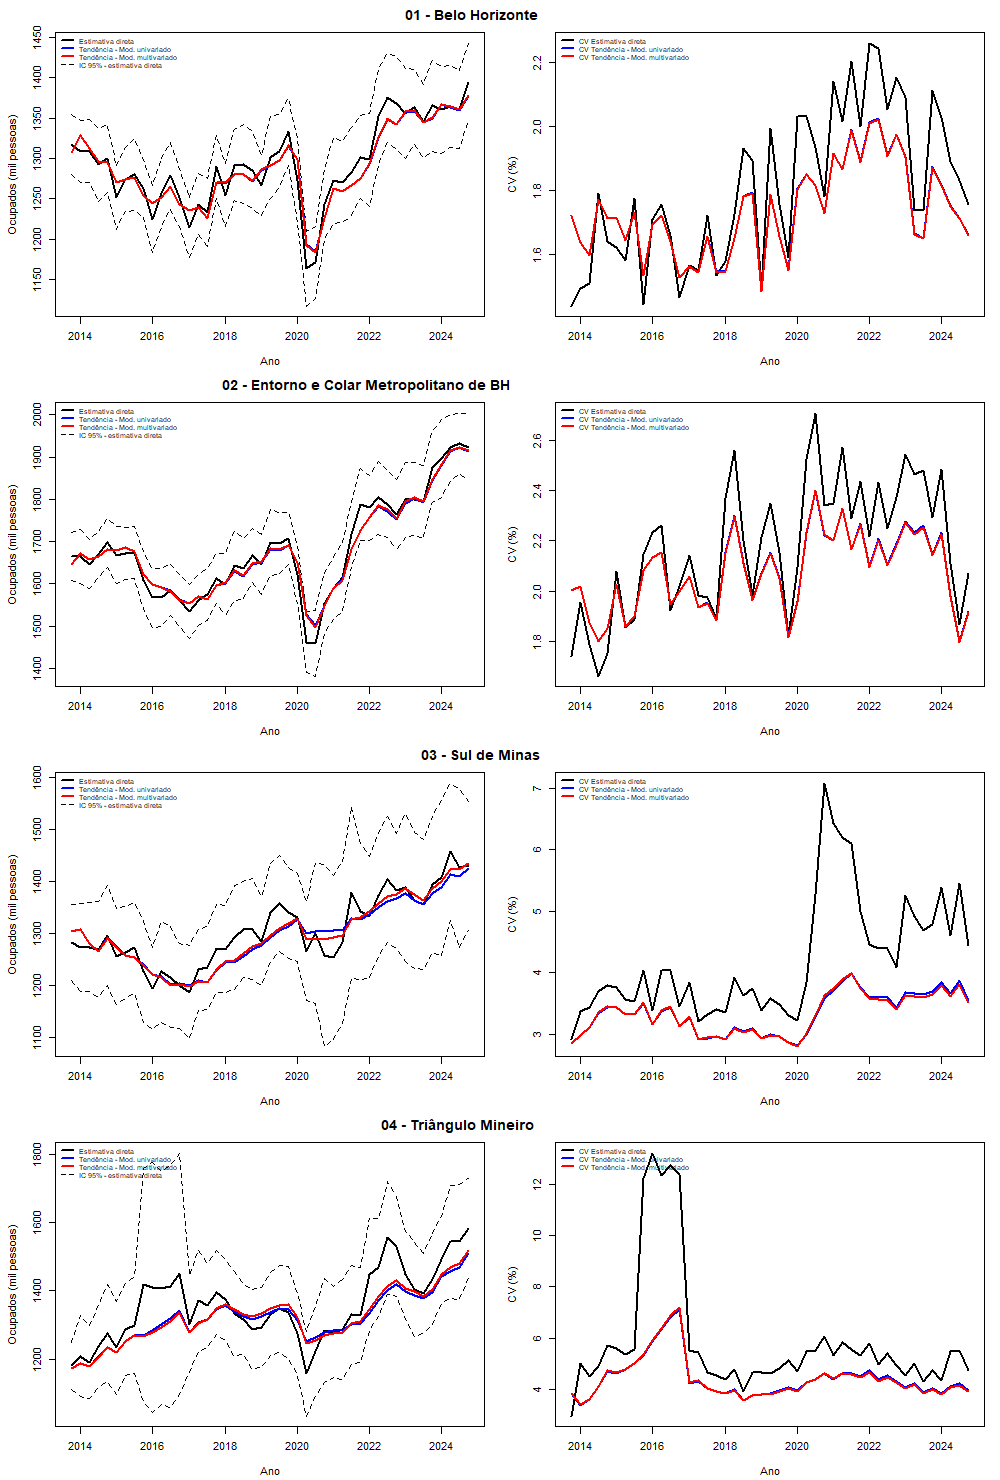
\includegraphics[width=0.85\linewidth]{resultados/Total de ocupados/Figura_Ocupacao_1.png}
    \fonte{Elaboração própria, com base nos dados da PNAD Contínua.}
    \label{fig:est_ocup_1}
\end{figure}

\begin{figure}[H]
    \centering
    \caption{Estimativas da tendência para o total de ocupados e respectivos coeficientes de variação -- regiões 5 a 8 -- 4º trimestre de 2013 ao 4º trimestre de 2024}
    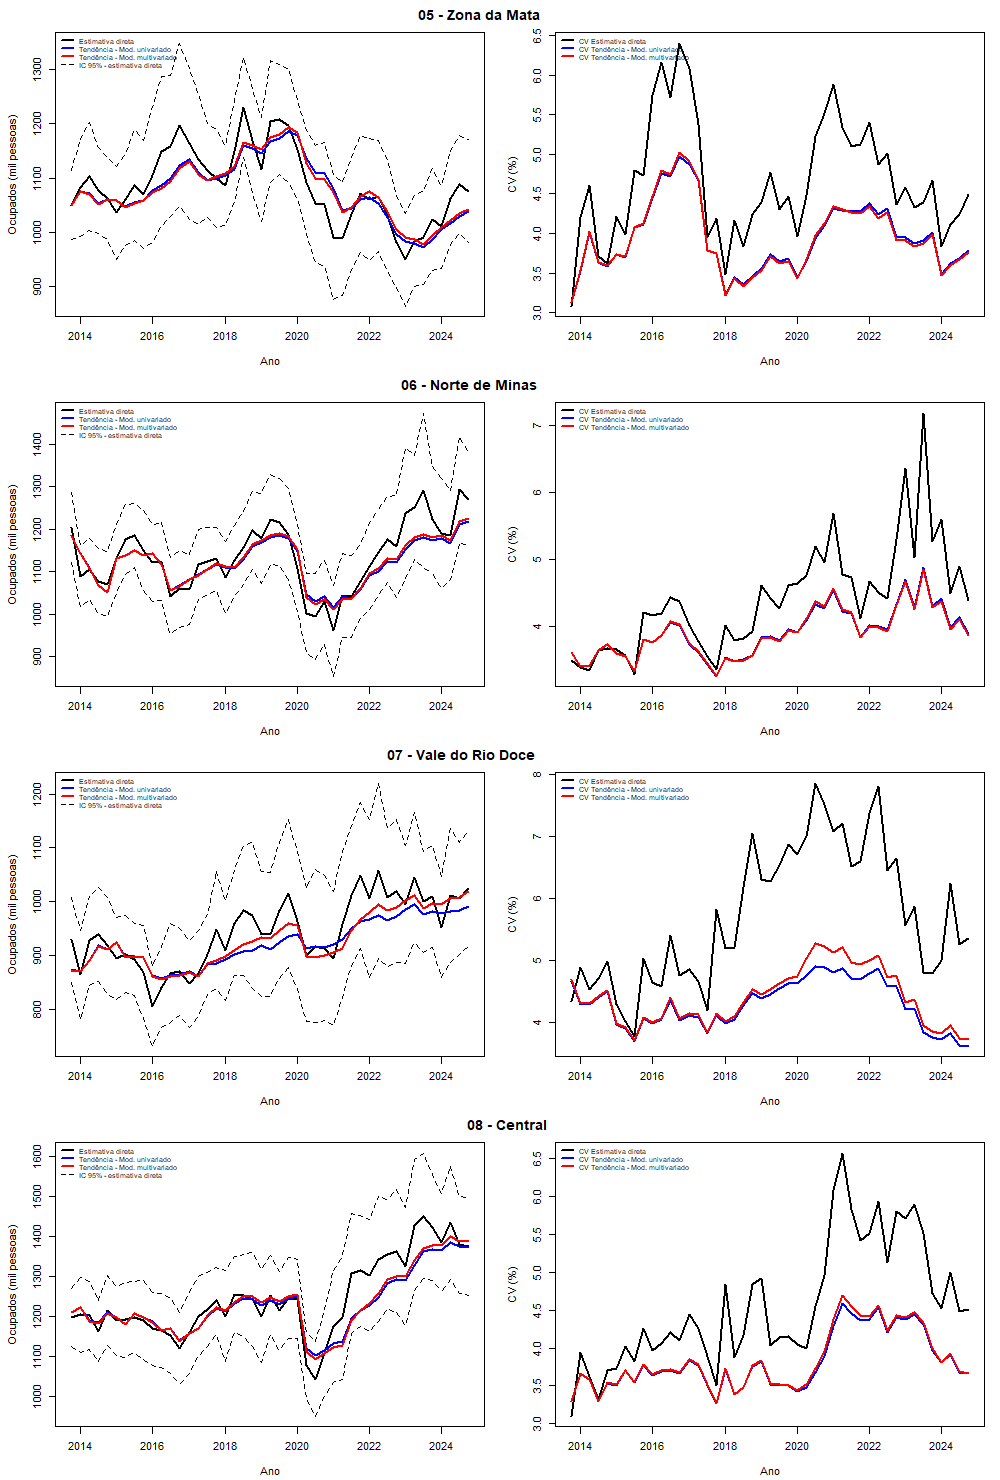
\includegraphics[width=0.85\linewidth]{resultados/Total de ocupados/Figura_Ocupacao_2.png}
    \fonte{Elaboração própria, com base nos dados da PNAD Contínua.}
    \label{fig:est_ocup_2}
\end{figure}
\vspace{-0.4cm}

Na Figura \ref{fig:est_ocup_2}, observa-se que as duas especificações produzem trajetórias praticamente sobrepostas em todos os quatro estratos, com diferenças de coeficiente de variação inferiores a 0,1 ponto percentual na Zona da Mata e na região Central. Essa coincidência é a expressão gráfica do resultado já registrado nas medidas de desempenho: para o total de ocupados, a informação tomada emprestada entre domínios é pequena.

Também se observa a presença de coeficientes de variação mais elevados no início das séries estimadas, sobretudo nas regiões 2, 4, 6 e 7. Esse comportamento está associado ao período inicial de estabilização do filtro de Kalman. Conforme \citet{durbinkoop2012}, recomenda-se cautela na interpretação das primeiras observações suavizadas, pois os resultados podem ser influenciados pela inicialização do vetor de estados. Por essa razão, as análises gráficas foram concentradas a partir do quarto trimestre de 2013.

Diferentemente do observado para o total de desocupados, a especificação multivariada não produziu ganho de precisão para o total de ocupados: o ganho médio foi de 14,9\% no modelo univariado e de 14,6\% no multivariado. Esse resultado é coerente com a estrutura de dependência estimada. Enquanto para os desocupados a matriz de covariância dos distúrbios das inclinações tem posto efetivo dois, indicando forte tendência comum a ser explorada, para os ocupados o posto efetivo é sete, de modo que há pouca informação a ser tomada emprestada entre os domínios. O contraste entre os dois indicadores é, em si, um resultado do artigo: o ganho da especificação multivariada não é automático, mas condicionado à existência de dependência de posto reduzido entre os domínios.

Adota-se, ainda assim, a especificação multivariada como principal também para o total de ocupados, por permitir o cálculo da taxa de desocupação a partir de componentes estimados sob uma mesma estrutura. Registra-se, contudo, que para este indicador a escolha é indiferente do ponto de vista da precisão.

A Tabela \ref{tab:pontual_ocup} apresenta os resultados pontuais do modelo multivariado para o último trimestre da série.

\vspace{-0.2cm}
\begin{table}[H]
\centering
\captionsetup{justification=centering}
\caption{Resultados pontuais do modelo multivariado para o total de ocupados - 4\textordmasculine{} trimestre de 2024}
\label{tab:pontual_ocup}

\renewcommand{\arraystretch}{0.8}
\resizebox{\textwidth}{!}{%
\begin{tabular}{@{}p{2.8cm}cccccc@{}}
\toprule
\textbf{Estrato Geográfico} & $\hat{y}$ & $CV(\hat{y})$ & IC 95\% & $\hat{\theta}$ & $CV(\hat{\theta})$ & IC 95\% \\
\midrule
01 - Belo Horizonte & 1394,54 & 1,76\% & [1346,53 ; 1442,54] & 1391,11 & 1,63\% & [1346,66 ; 1435,56] \\
\raisebox{0em}{\parbox[t]{4.3cm}{02 - Entorno e Colar \\[-2pt] Metropolitano de BH}} & 1923,78 & 2,07\% & [1845,68 ; 2001,89] & 1929,28 & 1,89\% & [1857,79 ; 2000,77] \\
03 - Sul de Minas & 1429,66 & 4,45\% & [1304,90 ; 1554,42] & 1433,20 & 3,51\% & [1334,72 ; 1531,68] \\
04 - Triângulo Mineiro & 1582,25 & 4,72\% & [1435,74 ; 1728,75] & 1523,33 & 3,89\% & [1407,31 ; 1639,34] \\
05 - Zona da Mata & 1075,88 & 4,49\% & [981,15 ; 1170,60] & 1043,06 & 3,78\% & [965,68 ; 1120,44] \\
06 - Norte de Minas & 1270,40 & 4,39\% & [1161,19 ; 1379,62] & 1231,96 & 3,82\% & [1139,62 ; 1324,31] \\
07 - Vale do Rio Doce & 1024,62 & 5,35\% & [917,08 ; 1132,16] & 1030,74 & 3,71\% & [955,69 ; 1105,78] \\
08 - Central & 1374,72 & 4,51\% & [1253,32 ; 1496,11] & 1389,45 & 3,66\% & [1289,85 ; 1489,05] \\
\bottomrule
\end{tabular}%
}
\fonte{Elaboração própria, com base nos dados da PNAD Contínua. Nota: \(\hat{y}\) é a estimativa direta e \(\hat{\theta}\) o sinal estimado pelo modelo multivariado (tendência mais sazonalidade). Valores em milhares de pessoas.}
\end{table}

\vspace{-0.3cm}

Observa-se ganho de precisão das estimativas baseadas em modelo em relação às estimativas diretas em todos os estratos, ainda que reduzido nos dois estratos metropolitanos. Mesmo em regiões cujas estimativas diretas já apresentavam coeficientes de variação inferiores a 5\%, o modelo foi capaz de filtrar o erro amostral, produzindo tendências mais estáveis.

\clearpage
\subsection{Taxa de desocupação}

A estimação da tendência da taxa de desocupação completa a análise dos indicadores regionais do mercado de trabalho mineiro. Para esse indicador, foram consideradas duas estratégias. A primeira consistiu no cálculo indireto da taxa a partir das tendências estimadas para o total de desocupados e o total de ocupados. A segunda consistiu na estimação direta da tendência da taxa de desocupação por meio do Modelo Estrutural Básico com erro amostral.

No primeiro caso, a tendência da taxa de desocupação, \(\hat{r}_L\), foi calculada a partir da tendência estimada do total de desocupados, \(\hat{D}_L\), e da tendência estimada do total de ocupados, \(\hat{O}_L\), conforme a Equação \ref{eq:tend_taxa}:

\vspace{-0.5cm}
\begin{equation}
    \hat{r}_L = \frac{\hat{D}_L}{\hat{D}_L+\hat{O}_L}.
    \label{eq:tend_taxa}
\end{equation}

\noindent
O denominador da Equação \ref{eq:tend_taxa} corresponde à tendência estimada da força de trabalho, \(T_L=\hat{D}_L+\hat{O}_L\). A variância aproximada de \(\hat{r}_L\) foi obtida por linearização de Taylor \citep{silva2021}:
\begin{equation}
    V(\hat{r}_L) =
    \frac{1}{T_L^2}V(\hat{D}_L)
    + \frac{\hat{D}_L^2}{T_L^4}V(T_L)
    - 2\frac{\hat{D}_L}{T_L^3}\mathrm{Cov}(\hat{D}_L,T_L).
    \label{eq:var_taxa}
\end{equation}

\noindent
Como simplificação operacional, e diante da ausência de uma estimativa direta da covariância entre os componentes suavizados, assumiu-se nula a covariância entre a tendência do total de desocupados e a tendência da força de trabalho. Assim, a variância aproximada pode ser escrita como:

\vspace{-0.5cm}
\begin{equation}
    V(\hat{r}_L) \approx
    \frac{1}{T_L^2}V(\hat{D}_L)
    + \frac{\hat{D}_L^2}{T_L^4}V(T_L).
    \label{eq:var_taxafinal}
\end{equation}
A hipótese \(\mathrm{Cov}(\hat{D}_L,T_L)=0\) merece registro, pois não é inócua. Desocupados e força de trabalho são positivamente associados na prática, de modo que o termo omitido na Equação \ref{eq:var_taxafinal} é positivo e entra subtraindo. A variância assim obtida tende, portanto, a ser uma \textit{sobre-estimativa} da variância verdadeira do cálculo indireto. Essa direção conhecida do viés é relevante para a comparação que se segue: ela opera a favor do cálculo indireto quando este é avaliado pelo vício, e contra ele quando avaliado pela precisão.

A segunda estratégia consistiu em estimar diretamente a taxa de desocupação por meio do Modelo Estrutural Básico com erro amostral. O procedimento seguiu as mesmas etapas aplicadas ao total de ocupados e ao total de desocupados: identificação individual do processo do erro amostral, estimação em ambiente univariado e multivariado, diagnóstico dos resíduos e avaliação do desempenho em relação à estimativa direta. Esses resultados complementares são apresentados no Apêndice A.

A Tabela \ref{tab:comptaxa} compara as duas estratégias. As Figuras \ref{fig:est_txdesoc_1} e \ref{fig:est_txdesoc_2} apresentam as tendências estimadas e os respectivos coeficientes de variação para cada estrato geográfico.

\vspace{-0.3cm}
\begin{table}[H]
\centering
\captionsetup{justification=centering}
\caption{Comparação entre as duas estratégias para a taxa de desocupação - cálculo indireto e estimação direta pelo modelo multivariado}
\label{tab:comptaxa}
{%
\renewcommand{\arraystretch}{0.8}
\scalebox{0.9}{%
\begin{tabular}{lccccc}
\toprule
& \multicolumn{3}{c}{\textbf{Coeficiente de variação médio (\%)}} & \multicolumn{2}{c}{\textbf{\makecell{Diferença relativa média \\ do erro padrão (\%)}}} \\
\cmidrule(lr){2-4} \cmidrule(lr){5-6}
\multicolumn{1}{l}{\textbf{Estrato Geográfico}} & \textbf{\makecell{Estimativa \\ direta}} & \textbf{\makecell{Cálculo \\ indireto}} & \textbf{\makecell{Modelo \\ direto}} & \textbf{\makecell{Cálculo \\ indireto}} & \textbf{\makecell{Modelo \\ direto}} \\
\midrule
01 - Belo Horizonte & 7,69 & 5,68 & 4,90 & 25,04 & 35,86 \\
02 - Entorno e Colar Metropolitano de BH & 7,33 & 5,82 & 4,95 & 19,04 & 31,30 \\
03 - Sul de Minas & 11,16 & 8,35 & 7,00 & 25,26 & 38,19 \\
04 - Triângulo Mineiro & 12,43 & 7,82 & 6,30 & 35,38 & 48,82 \\
05 - Zona da Mata & 10,84 & 10,29 & 8,27 & 4,34 & 23,33 \\
06 - Norte de Minas & 9,16 & 7,30 & 5,33 & 17,44 & 39,83 \\
07 - Vale do Rio Doce & 10,58 & 10,11 & 7,19 & 5,53 & 32,59 \\
08 - Central & 11,16 & 8,39 & 7,37 & 24,07 & 34,91 \\
\midrule
\textbf{Média} & \textbf{10,04} & \textbf{7,97} & \textbf{6,41} & \textbf{19,51} & \textbf{35,60} \\
\bottomrule
\end{tabular}%
}
}
\fonte{Elaboração própria, com base nos dados da PNAD Contínua. Nota: o cálculo indireto obtém a taxa a partir das tendências estimadas do total de desocupados e do total de ocupados, com variância por linearização de Taylor sob a hipótese \(\mathrm{Cov}(\hat{D}_L,T_L)=0\), discutida no texto. As oito primeiras observações foram descartadas do cálculo.}
\end{table}

\vspace{-0.4cm}
\begin{figure}[H]
    \centering
    \caption{Estimativas da tendência da taxa de desocupação e respectivos coeficientes de variação -- regiões 1 a 4 -- 1º trimestre de 2014 ao 4º trimestre de 2024}
    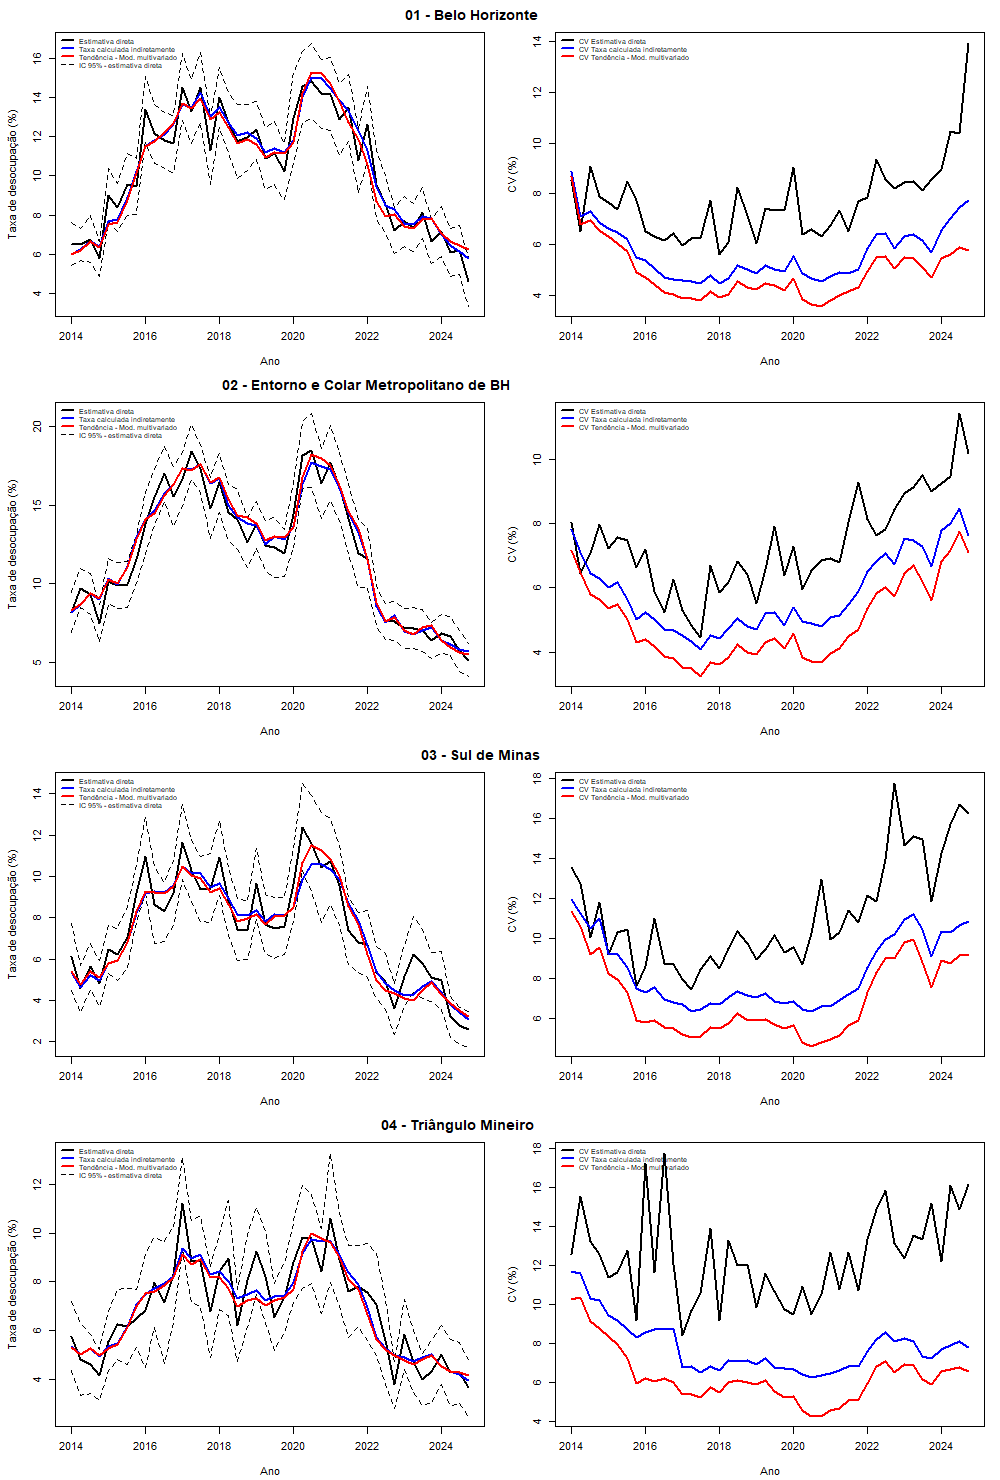
\includegraphics[width=0.85\linewidth]{resultados/Taxa de desocupação/Figura_TaxaDesoc_1.png}
    \fonte{Elaboração própria, com base nos dados da PNAD Contínua.}
    \label{fig:est_txdesoc_1}
\end{figure}

\begin{figure}[H]
    \centering
    \caption{Estimativas da tendência da taxa de desocupação e respectivos coeficientes de variação -- regiões 5 a 8 -- 1º trimestre de 2014 ao 4º trimestre de 2024}
    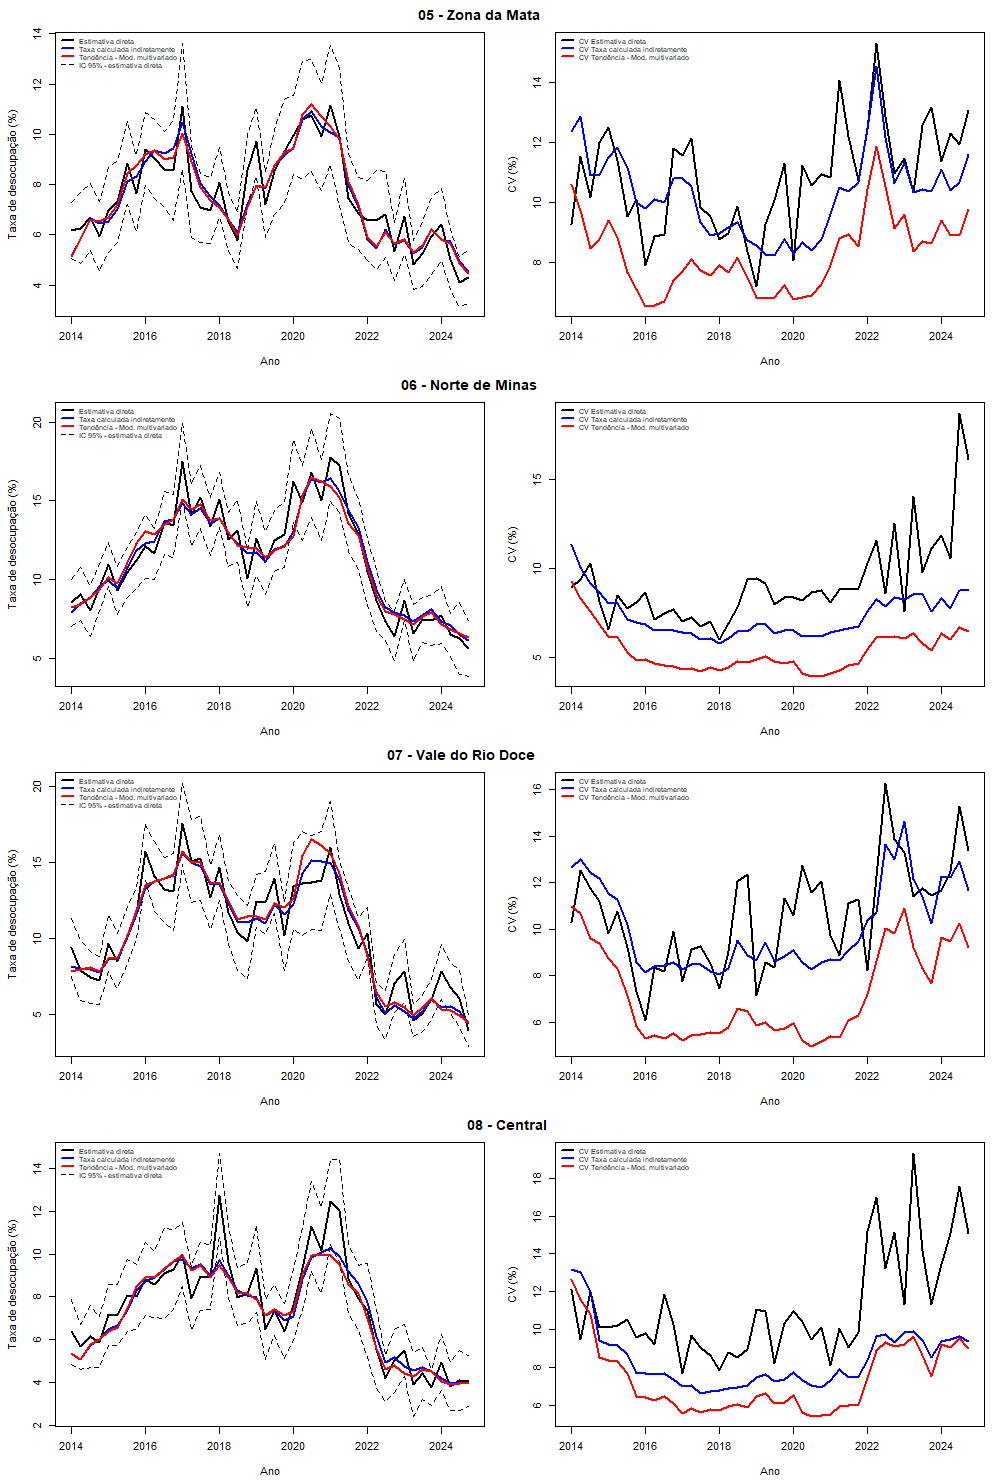
\includegraphics[width=0.85\linewidth]{resultados/Taxa de desocupação/Figura_TaxaDesoc_2.png}
    \fonte{Elaboração própria, com base nos dados da PNAD Contínua.}
    \label{fig:est_txdesoc_2}
\end{figure}

Do ponto de vista regional, as tendências estimadas indicam que a dinâmica da desocupação não foi homogênea entre os estratos mineiros. Embora todas as regiões tenham sido afetadas pelos ciclos de deterioração e recuperação do mercado de trabalho observados no período, a intensidade e a persistência desses movimentos diferem entre os estratos. Essa heterogeneidade reforça a limitação de análises baseadas apenas no agregado estadual e evidencia a relevância de indicadores regionais mais precisos para o acompanhamento conjuntural do mercado de trabalho.

Assim como nas demais variáveis, o sinal estimado para a taxa de desocupação permaneceu dentro dos intervalos de confiança de 95\% das estimativas diretas em 346 dos 352 pontos analisados, ou seja, em 98,3\% dos casos. Esse resultado indica que os modelos preservam a trajetória observada nas estimativas diretas, ao mesmo tempo em que produzem séries mais estáveis. As tendências captaram os principais momentos de deterioração e recuperação do mercado de trabalho, incluindo a crise econômica de 2015--2016 e os efeitos associados à crise sanitária da Covid-19.

Em relação à precisão, tanto a taxa calculada indiretamente quanto a tendência estimada diretamente por modelo apresentaram coeficientes de variação inferiores aos das estimativas diretas na maior parte do período e dos estratos. As principais exceções ocorreram nas observações iniciais das séries do Sul de Minas, da Zona da Mata e da região Central, período em que a influência da inicialização do filtro de Kalman ainda é mais relevante.

A comparação entre as duas estratégias é inequívoca em favor da estimação direta. O coeficiente de variação médio das estimativas diretas do desenho é de 10,0\%; o cálculo indireto o reduz para 8,0\% e o modelo multivariado aplicado à própria taxa, para 6,4\%. Em termos de diferença relativa média do erro-padrão, o ganho é de 19,5\% no cálculo indireto e de 35,6\% na estimação direta, e a estimação direta supera o cálculo indireto \textit{em todos os oito estratos}, sem exceção. A vantagem é particularmente expressiva na Zona da Mata (23,3\% contra 4,3\%) e no Vale do Rio Doce (32,6\% contra 5,5\%), justamente os estratos em que o cálculo indireto pouco contribui.

Cabe registrar que esse resultado não decorre apenas do desempenho superior do modelo direto, mas também de uma fragilidade do cálculo indireto: por depender das tendências de desocupados e de ocupados, ele herda o fraco desempenho da especificação multivariada para o total de ocupados, além de repousar sobre a hipótese \(\mathrm{Cov}(\hat{D}_L,T_L)=0\), cuja violação, como discutido, infla a variância calculada. A estimação direta não depende de nenhuma dessas duas condições.

Adota-se, portanto, a estimação direta pelo modelo multivariado como estratégia de referência para a taxa de desocupação. O cálculo indireto é reportado como alternativa, com duas qualidades próprias que justificam mantê-lo no texto: é mais simples de implementar e assegura, por construção, coerência aritmética entre os três indicadores publicados --- propriedade que a estimação direta não garante, uma vez que a tendência da taxa é estimada independentemente das tendências de seus componentes.

Em conjunto, os resultados mostram que o agregado estadual oculta trajetórias regionais distintas no mercado de trabalho mineiro. As estimativas baseadas em modelo permitem acompanhar essas diferenças com menor variabilidade amostral, especialmente nos estratos em que as estimativas diretas apresentam maior instabilidade. Esse resultado é relevante para o desenho e o monitoramento de políticas públicas, pois indica que diagnósticos baseados apenas no nível estadual podem subestimar ou suavizar movimentos específicos de deterioração e recuperação em determinadas regiões.

\section{Conclusão}
\label{sec:conclusão}

Este artigo analisou as tendências do total de desocupados, do total de ocupados e da taxa de desocupação nos estratos geográficos de Minas Gerais, com base nas séries trimestrais da PNAD Contínua. O estudo partiu do problema da escassez de indicadores regionais consistentes para o acompanhamento do mercado de trabalho em recortes intraestaduais, especialmente em domínios nos quais as estimativas diretas apresentam maior variabilidade amostral.

Para isso, foi aplicado o Modelo Estrutural Básico com incorporação explícita do erro amostral. O componente estrutural permitiu decompor o parâmetro populacional das séries em tendência, sazonalidade e componente irregular \citep{harvey1989}. O componente de erro amostral, por sua vez, permitiu considerar a dependência temporal induzida pelo desenho da PNAD Contínua e por sua estrutura de sobreposição amostral \citep{scott1974,scott1977}.

Além da estimação direta da taxa de desocupação, o artigo também avaliou uma alternativa indireta, calculada a partir das tendências estimadas para o total de desocupados e o total de ocupados. A comparação foi conclusiva em favor da estimação direta, que apresentou ganho médio de precisão de 35,6\% contra 19,5\% do cálculo indireto e superou a alternativa em todos os oito estratos. O cálculo indireto permanece registrado como opção, por sua simplicidade e por assegurar coerência aritmética entre os indicadores publicados.

Os resultados indicaram que as estimativas baseadas em modelo apresentaram maior precisão do que as estimativas diretas da PNAD Contínua, com ganhos de magnitude bastante desigual entre os indicadores. Para o total de desocupados, o ganho médio foi de 32,7\% na especificação multivariada, com coeficientes de variação sistematicamente menores e preservação da trajetória observada nas estimativas diretas. Para a taxa de desocupação, o ganho médio foi de 35,6\%. Para o total de ocupados, contudo, o ganho médio limitou-se a 14,6\%, concentrado nos estratos do interior, uma vez que nas duas regiões metropolitanas a estimativa direta já é bastante precisa.

A comparação entre modelos univariados e multivariados produziu o que talvez seja o resultado metodológico mais informativo do artigo: o ganho da formulação multivariada não é automático, mas condicionado à estrutura de dependência entre os domínios. Para o total de desocupados e para a taxa, cuja matriz de covariância dos distúrbios das inclinações tem posto efetivo dois, a especificação multivariada praticamente triplicou o ganho de precisão em relação à univariada. Para o total de ocupados, cujo posto efetivo é sete, os dois modelos são equivalentes. A dependência de posto reduzido entre os estratos é, portanto, a condição que torna vantajoso tomar informação emprestada entre domínios --- e essa condição precisa ser verificada, não presumida.

Do ponto de vista substantivo, os resultados contribuem para o acompanhamento regionalizado do mercado de trabalho mineiro. As tendências estimadas permitiram identificar a evolução dos indicadores nos diferentes estratos, preservando os movimentos observados nas estimativas diretas, mas reduzindo a volatilidade associada ao erro amostral. Dessa forma, a abordagem proposta oferece uma alternativa relevante para a produção de estatísticas em pequenos domínios, especialmente quando se trabalha com séries temporais relativamente curtas e com amostras efetivas reduzidas.

O estudo possui limitações. A primeira refere-se à agregação de dois estratos originais da PNAD Contínua, resultando em oito regiões de análise. Essa decisão foi justificada pela elevada imprecisão das estimativas diretas na RIDE de Brasília em Minas e no Colar Metropolitano de Belo Horizonte, mas implica perda de detalhamento territorial. A segunda limitação decorre do escopo dos indicadores analisados, restritos ao total de ocupados, ao total de desocupados e à taxa de desocupação, sem desagregações por sexo, idade, escolaridade ou outras características sociodemográficas.

Uma terceira limitação refere-se ao fato de que as estimativas produzidas para os estratos não foram submetidas a procedimentos de \textit{benchmarking} ou reconciliação com estimativas agregadas para Minas Gerais. Assim, embora o foco do artigo esteja na precisão e na estabilidade das séries regionais, permanece como agenda metodológica a compatibilização formal entre estimativas de diferentes níveis territoriais.

Três limitações de natureza propriamente estatística devem ser registradas de forma explícita. A primeira é a fraca identificação da variância do componente irregular: o perfil de verossimilhança é quase plano em \(\sigma_I^2\) --- multiplicar essa variância por cem altera a log-verossimilhança em menos de \(10^{-5}\) na mediana dos casos, contra o limiar de 1,92 de um teste a 5\% ---, a estimativa resultante é praticamente nula em todos os estratos e indicadores e, por consequência, a série dessazonalizada coincide com a tendência estimada. O modelo, tal como especificado, não separa empiricamente tendência e choques transitórios, e este artigo não apresenta séries dessazonalizadas como produto autônomo.

O mesmo diagnóstico se aplica, com uma exceção, à variância do componente sazonal: a sazonalidade é efetivamente determinística em 23 das 24 combinações de estrato e indicador. A exceção é a taxa de desocupação no Norte de Minas, único caso em que \(\sigma_S^2\) é fortemente identificada, com variação de 26,9 na log-verossimilhança sob a mesma perturbação.

A segunda limitação é a rejeição da hipótese de normalidade dos resíduos em cinco dos oito estratos no total de ocupados, associada às observações atípicas de 2020. Os intervalos de confiança desse indicador devem, por isso, ser lidos com cautela, e o tratamento das observações da pandemia por variáveis de intervenção permanece como agenda.

A terceira é a autocorrelação serial remanescente, restrita a dois casos isolados no modelo multivariado: o Norte de Minas no total de desocupados (\(p=0{,}001\)) e o Colar e Entorno Metropolitano de BH no total de ocupados (\(p=0{,}042\)). Para a taxa de desocupação, indicador de referência do artigo, nenhum estrato rejeita a hipótese de brancura dos resíduos no modelo multivariado. Registre-se, por fim, que o esquema de rotação da PNAD Contínua induz também um viés de grupo de rotação, cujo tratamento explícito não foi incorporado a este artigo e constitui extensão natural do modelo aqui apresentado.
Como extensão futura, sugere-se ampliar a aplicação para estratos geográficos de outras unidades da federação, especialmente estados limítrofes a Minas Gerais, permitindo investigar interações regionais mais amplas nos mercados de trabalho. Do ponto de vista metodológico, uma agenda promissora consiste em incorporar procedimentos de \textit{benchmarking}, de modo a compatibilizar as estimativas dos estratos com totais conhecidos em níveis territoriais mais agregados \citep{pfeffermann2006}. Também seria relevante explorar modelos multivariados com recortes sociodemográficos, desde que a qualidade das estimativas diretas permita essa ampliação.

Por fim, espera-se que os resultados contribuam para a discussão sobre o uso de modelos de séries temporais na produção de estatísticas regionais. Ao demonstrar ganhos de precisão em indicadores da PNAD Contínua para pequenos domínios, o artigo reforça a relevância de metodologias baseadas em modelo como complemento à abordagem tradicional baseada no desenho amostral. Essa combinação é particularmente importante em contextos nos quais a demanda por informações territoriais desagregadas cresce mais rapidamente do que a capacidade de ampliação das amostras, como ocorre no acompanhamento regional do mercado de trabalho.

\bibliographystyle{econbr.bst} % Style BST file
\bibliography{bibliography.bib}  % Bibliography file

\clearpage
\appendix
\section{Resultados complementares dos modelos da Taxa de Desocupação}

\vspace{-0.2cm}
\begin{table}[H]
\centering
\captionsetup{justification=centering}
\caption{Hiperparâmetros estimados para a taxa de desocupação - modelos univariado e multivariado}
\label{tab:hipertaxa}
\scalebox{0.92}{
\renewcommand{\arraystretch}{0.85}
\begin{tabular}{llccccc}
\toprule
& & \multicolumn{5}{c}{\textbf{Modelo Univariado}} \\
\cmidrule(lr){3-7}
\textbf{Estrato geográfico} & \textbf{Processo} & \(\hat{\sigma}_L^2\) & \(\hat{\sigma}_R^2\) & \(\hat{\sigma}_S^2\) & \(\hat{\sigma}_I^2\) & \(\hat{\sigma}_{\tilde{e}}^2\) \\
\midrule
01 - Belo Horizonte & AR(1) & 0,0000 & 0,1028 & 0,0000 & 0,0000 & 0,9263 \\
02 - Entorno e Colar Metropolitano de BH & MA(1) & 0,0000 & 0,3350 & 0,0000 & 0,0000 & 0,9485 \\
03 - Sul de Minas & AR(1) & 0,5334 & 0,0051 & 0,0000 & 0,0000 & 0,8744 \\
04 - Triângulo Mineiro & AR(1) & 0,0000 & 0,0431 & 0,0000 & 0,0000 & 0,9604 \\
05 - Zona da Mata & AR(1) & 0,3514 & 0,0023 & 0,0000 & 0,0000 & 0,9584 \\
06 - Norte de Minas & MA(1) & 0,1873 & 0,1890 & 0,0091 & 0,0000 & 0,8083 \\
07 - Vale do Rio Doce & AR(1) & 1,0321 & 0,0100 & 0,0000 & 0,0000 & 0,8583 \\
08 - Central & AR(3) & 0,0003 & 0,1653 & 0,0000 & 0,0000 & 0,8978 \\
\midrule
& & \multicolumn{5}{c}{\textbf{Modelo Multivariado}} \\
\cmidrule(lr){3-7}
\textbf{Estrato geográfico} & \textbf{Processo} & \(\hat{\sigma}_L^2\) & \(\hat{\sigma}_R^2\) & \(\hat{\sigma}_S^2\) & \(\hat{\sigma}_I^2\) & \(\hat{\sigma}_{\tilde{e}}^2\) \\
\midrule
01 - Belo Horizonte & AR(1) & 0,0000 & 0,2211 & 0,0000 & 0,0000 & 0,9263 \\
02 - Entorno e Colar Metropolitano de BH & MA(1) & 0,0000 & 0,3694 & 0,0000 & 0,0000 & 0,9485 \\
03 - Sul de Minas & AR(1) & 0,0004 & 0,1506 & 0,0000 & 0,0000 & 0,8744 \\
04 - Triângulo Mineiro & AR(1) & 0,0000 & 0,0876 & 0,0000 & 0,0000 & 0,9604 \\
05 - Zona da Mata & AR(1) & 0,0055 & 0,0814 & 0,0000 & 0,0000 & 0,9584 \\
06 - Norte de Minas & MA(1) & 0,0017 & 0,2484 & 0,0099 & 0,0000 & 0,8083 \\
07 - Vale do Rio Doce & AR(1) & 0,0016 & 0,3222 & 0,0000 & 0,0000 & 0,8583 \\
08 - Central & AR(3) & 0,0003 & 0,1245 & 0,0000 & 0,0000 & 0,8978 \\
\bottomrule
\end{tabular}}
\fonte{Elaboração própria, com base nos dados da PNAD Contínua. Nota: o processo do erro amostral é identificado individualmente por estrato (Seção \ref{sec:metodologia}), e \(\hat{\sigma}_{\tilde{e}}^2\) é derivada dos coeficientes do processo, por isso coincidindo nos dois modelos. Sobre \(\sigma_I^2\), ver a ressalva de identificação no texto.}
\end{table}

\vspace{-0.3cm}

\vspace{-0.2cm}
\begin{table}[H]
\centering
\captionsetup{justification=centering}
\caption{Teste de diagnóstico do resíduo para a taxa de desocupação - modelos univariado e multivariado}
\label{tab:diagtaxa}
\scalebox{1}{
\renewcommand{\arraystretch}{0.7}
\begin{tabular}{lccc}
\toprule
& \multicolumn{3}{c}{\textbf{Modelo Univariado}} \\
\cmidrule(lr){2-4}
\textbf{Estrato geográfico} & Shapiro-Wilk & Ljung-Box & H \\
\midrule
01 - Belo Horizonte & 0,8601 & 0,9309 & 0,5742 \\
02 - Entorno e Colar Metropolitano de BH & 0,1700 & 0,0319** & 0,6347 \\
03 - Sul de Minas & 0,0512* & 0,0799* & 0,9262 \\
04 - Triângulo Mineiro & 0,6179 & 0,2440 & 0,8540 \\
05 - Zona da Mata & 0,9283 & 0,2884 & 0,6149 \\
06 - Norte de Minas & 0,1454 & 0,0974* & 0,5049 \\
07 - Vale do Rio Doce & 0,8520 & 0,3597 & 0,2295 \\
08 - Central & 0,1325 & 0,1337 & 0,1126 \\
\midrule
& \multicolumn{3}{c}{\textbf{Modelo Multivariado}} \\
\cmidrule(lr){2-4}
\textbf{Estrato geográfico} & Shapiro-Wilk & Ljung-Box & H \\
\midrule
01 - Belo Horizonte & 0,8407 & 0,8420 & 0,5084 \\
02 - Entorno e Colar Metropolitano de BH & 0,6037 & 0,0951* & 0,6204 \\
03 - Sul de Minas & 0,3230 & 0,1650 & 0,9349 \\
04 - Triângulo Mineiro & 0,9237 & 0,2139 & 0,3977 \\
05 - Zona da Mata & 0,0237** & 0,3745 & 0,9795 \\
06 - Norte de Minas & 0,2102 & 0,4442 & 0,3363 \\
07 - Vale do Rio Doce & 0,4342 & 0,4100 & 0,2346 \\
08 - Central & 0,6965 & 0,6044 & 0,4538 \\
\bottomrule
\end{tabular}}
\fonte{Elaboração própria, com base nos dados da PNAD Contínua. Nota: * representa rejeição de \(H_0\) a 10\%, ** a 5\% e *** a 1\%. As oito primeiras observações foram descartadas, em razão do período de estabilização do filtro de Kalman.}
\end{table}

\vspace{-0.3cm}

\vspace{-0.2cm}
\begin{table}[H]
\centering
\captionsetup{justification=centering}
\caption{Correlação estimada entre os distúrbios das inclinações - modelo multivariado - taxa de desocupação}
\label{tab:matriz_correlacao_taxa}

\renewcommand{\arraystretch}{0.8}

\resizebox{\linewidth}{!}{%
\begin{tabular}{@{}p{2.8cm}c*{8}{c}@{}}
\toprule
\textbf{Estrato Geográfico} & \(\hat{\sigma}_R^2\) & \textbf{1} & \textbf{2} & \textbf{3} & \textbf{4} & \textbf{5} & \textbf{6} & \textbf{7} & \textbf{8} \\
\midrule
01 - Belo Horizonte & 0,2211 & 1 &  &  &  &  &  &  &  \\
\raisebox{0em}{\parbox[t]{2.8cm}{02 - Entorno e Colar \\[-2pt] Metropolitano de BH}} & 0,3694 & 1,0000 & 1 &  &  &  &  &  &  \\
03 - Sul de Minas & 0,1506 & 0,9878 & 0,9879 & 1 &  &  &  &  &  \\
04 - Triângulo Mineiro & 0,0876 & 0,9970 & 0,9971 & 0,9966 & 1 &  &  &  &  \\
05 - Zona da Mata & 0,0814 & 0,7292 & 0,7298 & 0,8249 & 0,7755 & 1 &  &  &  \\
06 - Norte de Minas & 0,2484 & 0,9953 & 0,9954 & 0,9982 & 0,9997 & 0,7899 & 1 &  &  \\
07 - Vale do Rio Doce & 0,3222 & 0,9828 & 0,9830 & 0,9995 & 0,9940 & 0,8390 & 0,9961 & 1 &  \\
08 - Central & 0,1245 & 0,9969 & 0,9969 & 0,9791 & 0,9923 & 0,6932 & 0,9891 & 0,9738 & 1 \\
\bottomrule
\end{tabular}%
}

\fonte{Elaboração própria, com base nos dados da PNAD Contínua. Nota: autovalores estimados de \(\Sigma_R\): 1,563; 0,041 e 6 valores inferiores a \(10^{-3}\). Posto numérico de 5 em 8; posto \textbf{efetivo} de 2, contando os autovalores que retêm ao menos 1\% do maior. As correlações devem, portanto, ser lidas em conjunto, e não isoladamente.}
\end{table}

\vspace{-0.3cm}

\vspace{-0.2cm}
\begin{table}[H]
\centering
\captionsetup{justification=centering}
\caption{Medidas de desempenho dos modelos univariado e multivariado - taxa de desocupação}
\label{tab:diffviciotaxa}
{%
\renewcommand{\arraystretch}{0.8}
\scalebox{0.95}{%
\begin{tabular}{lcccc}
\toprule
& \multicolumn{2}{c}{\textbf{\makecell{Diferença relativa média \\ do erro padrão (\%)}}} & \multicolumn{2}{c}{\textbf{Vício relativo (\%)}} \\
\cmidrule(lr){2-3} \cmidrule(lr){4-5}
\multicolumn{1}{l}{\textbf{Estrato Geográfico}} & \textbf{Univariado} & \textbf{Multivariado} & \textbf{Univariado} & \textbf{Multivariado} \\
\midrule
01 - Belo Horizonte & 11,93 & 35,86 & -0,04 & -0,53 \\
02 - Entorno e Colar Metropolitano de BH & 7,58 & 31,30 & 0,22 & 1,75 \\
03 - Sul de Minas & 8,78 & 38,19 & -0,50 & -2,54 \\
04 - Triângulo Mineiro & 20,70 & 48,82 & -0,14 & -1,75 \\
05 - Zona da Mata & 17,39 & 23,33 & -0,47 & -0,31 \\
06 - Norte de Minas & 3,88 & 39,83 & 0,05 & -0,65 \\
07 - Vale do Rio Doce & 7,28 & 32,59 & -0,29 & -0,12 \\
08 - Central & 8,46 & 34,91 & -0,80 & -3,37 \\
\midrule
\textbf{Média} & \textbf{10,75} & \textbf{35,60} & & \\
\bottomrule
\end{tabular}%
}
}
\fonte{Elaboração própria, com base nos dados da PNAD Contínua. Nota: as oito primeiras observações de cada série foram descartadas do cálculo, em razão do período de estabilização do filtro de Kalman.}
\end{table}

\vspace{-0.3cm}

\vspace{-0.2cm}
\begin{table}[H]
\centering
\captionsetup{justification=centering}
\caption{Resultados pontuais do modelo multivariado para a taxa de desocupação - 4\textordmasculine{} trimestre de 2024}
\label{tab:pontual_taxa}

\renewcommand{\arraystretch}{0.8}
\resizebox{\linewidth}{!}{%
\begin{tabular}{@{}p{2.8cm}cccccc@{}}
\toprule
\textbf{Estrato Geográfico} & $\hat{y}$ & $CV(\hat{y})$ & IC 95\% & $\hat{\theta}$ & $CV(\hat{\theta})$ & IC 95\% \\
\midrule
01 - Belo Horizonte & 4,59 & 13,92\% & [3,34 ; 5,84] & 5,37 & 6,82\% & [4,66 ; 6,09] \\
\raisebox{0em}{\parbox[t]{2.8cm}{02 - Entorno e Colar \\[-2pt] Metropolitano de BH}} & 5,16 & 10,16\% & [4,13 ; 6,18] & 4,69 & 8,29\% & [3,93 ; 5,45] \\
03 - Sul de Minas & 2,61 & 16,25\% & [1,78 ; 3,44] & 2,82 & 10,53\% & [2,24 ; 3,40] \\
04 - Triângulo Mineiro & 3,69 & 16,16\% & [2,52 ; 4,85] & 3,57 & 8,24\% & [3,00 ; 4,15] \\
05 - Zona da Mata & 4,31 & 13,05\% & [3,21 ; 5,41] & 4,26 & 10,39\% & [3,40 ; 5,13] \\
06 - Norte de Minas & 5,63 & 16,14\% & [3,85 ; 7,41] & 5,77 & 9,08\% & [4,74 ; 6,79] \\
07 - Vale do Rio Doce & 3,98 & 13,39\% & [2,94 ; 5,03] & 3,88 & 10,63\% & [3,07 ; 4,69] \\
08 - Central & 4,07 & 15,09\% & [2,86 ; 5,27] & 3,53 & 10,34\% & [2,82 ; 4,25] \\
\bottomrule
\end{tabular}%
}
\fonte{Elaboração própria, com base nos dados da PNAD Contínua. Nota: \(\hat{y}\) é a estimativa direta e \(\hat{\theta}\) o sinal estimado pelo modelo multivariado (tendência mais sazonalidade). Valores em pontos percentuais.}
\end{table}

\vspace{-0.3cm}

\end{document}
